% ==================================================================
% 4 RESULTADOS
% ==================================================================

\chapter{RESULTADOS}

\section{SELEÇÃO DA AMOSTRA DE ATIVOS}

A aplicação dos critérios metodológicos estabelecidos à base de dados da Economática, contendo 508 empresas listadas na B3, resultou na seleção de 10 ativos para compor as carteiras analisadas neste estudo.

\subsection{Aplicação dos Filtros Eliminatórios}

Dos 508 ativos disponíveis na base Economática, a aplicação sequencial dos filtros eliminatórios resultou em:

\begin{itemize}
    \item \textbf{Filtro de sobrevivência empresarial:} Foram removidos 47 ativos que apresentaram processos de falência, recuperação judicial ou delisting durante o período 2018-2019, restando 461 empresas;
    
    \item \textbf{Filtro de liquidez mínima:} Foram eliminados 398 ativos com volume médio diário inferior a R\$ 50 milhões no período 2016-2017, restando 63 empresas que atenderam ao critério de liquidez;
    
    \item \textbf{Filtro de disponibilidade de dados:} Foram removidos 8 ativos com mais de 5\% de dias sem negociação no período 2018-2019, resultando em 55 empresas elegíveis para a seleção final.
\end{itemize}

A alta taxa de eliminação (89,2\% dos ativos originais) reflete as características concentradas do mercado brasileiro, onde um pequeno grupo de empresas de grande porte concentra a maior parte da liquidez e do volume negociado.

\subsection{Ativos Selecionados}

A partir dos 55 ativos elegíveis, foram selecionados 10 ativos aplicando-se os critérios de representatividade de mercado, diversificação setorial e capitalização, conforme apresentado na Tabela \ref{tab:ativos_selecionados_performance}.

\begin{table}[H]
\centering
\caption{Ativos Selecionados para Análise - Características e Performance}
\begin{tabular}{|p{1.5cm}|p{4.5cm}|p{2.5cm}|p{1.8cm}|p{1.5cm}|p{1.3cm}|}
\hline
\textbf{Código} & \textbf{Empresa} & \textbf{Setor} & \textbf{Vol. Médio} & \textbf{Cap.} & \textbf{Ret.} \\
& & \textbf{Economática} & \textbf{(R\$ mi/dia)} & \textbf{(R\$ bi)} & \textbf{2018-19} \\
\hline
PETR4 & Petróleo Brasileiro S.A. & Petróleo e Gás & 1.247,3 & 198,5 & 26,12\% \\
\hline
VALE3 & Vale S.A. & Mineração & 982,1 & 165,2 & 16,56\% \\
\hline
ITUB4 & Itaú Unibanco Holding S.A. & Finanças e Seguros & 756,8 & 142,8 & 10,72\% \\
\hline
BBDC4 & Banco Bradesco S.A. & Finanças e Seguros & 432,9 & 89,6 & 12,95\% \\
\hline
ABEV3 & Ambev S.A. & Bebidas & 378,2 & 78,3 & -5,42\% \\
\hline
B3SA3 & B3 S.A. - Brasil, Bolsa, Balcão & Finanças e Seguros & 289,5 & 67,1 & 28,71\% \\
\hline
WEGE3 & WEG S.A. & Máquinas e Equipamentos & 198,7 & 45,2 & 35,25\% \\
\hline
RENT3 & Localiza Rent a Car S.A. & Outros Serviços & 156,3 & 38,9 & 35,42\% \\
\hline
LREN3 & Lojas Renner S.A. & Comércio & 134,5 & 32,4 & 26,95\% \\
\hline
ELET3 & Centrais Elétricas Brasileiras & Energia Elétrica & 89,7 & 28,6 & 16,52\% \\
\hline
\end{tabular}
\textit{Notas: Volume médio 2016-2017. Cap. Mercado jan/2018. Ret. = Retorno anualizado 2018-2019.}
\label{tab:ativos_selecionados_performance}
\end{table}

\subsection{Características da Amostra Final}

A amostra final apresenta diversificação adequada tanto em termos setoriais quanto de capitalização de mercado. O conjunto inclui empresas de setores estratégicos da economia brasileira, sendo 3 empresas do setor financeiro (ITUB4, BBDC4, B3SA3), 2 commodities (PETR4, VALE3) e 5 empresas de diferentes setores (bebidas, máquinas, serviços, varejo e energia elétrica).

A concentração em empresas de grande capitalização reflete a estrutura do mercado brasileiro, onde um pequeno número de blue chips concentra a maior parte da liquidez. Todas as empresas selecionadas eram representativas do mercado acionário nacional, tendo sido escolhidas com base em critérios de liquidez e capitalização estabelecidos ex-ante.

\section{ESTATÍSTICAS DESCRITIVAS DOS ATIVOS}

\subsection{Implementação Computacional}

O processamento dos dados foi realizado utilizando a linguagem Python, com as bibliotecas pandas para manipulação de dados, NumPy para cálculos matemáticos e matplotlib/seaborn para visualizações. Os retornos foram calculados utilizando a fórmula logarítmica para garantir aditividade temporal:

\begin{equation}
R_t = \ln\left(\frac{P_t}{P_{t-1}}\right)
\end{equation}

onde $R_t$ é o retorno no período $t$, $P_t$ é o preço no período $t$ e $P_{t-1}$ é o preço no período anterior. A anualização dos retornos e volatilidades seguiu as fórmulas padrão de finanças quantitativas, considerando 12 períodos mensais por ano.

\subsection{Análise dos Retornos e Volatilidades}

A Tabela \ref{tab:estatisticas_descritivas} apresenta as estatísticas descritivas completas dos 10 ativos selecionados, calculadas automaticamente pelo sistema desenvolvido em Python.

% Tabela gerada automaticamente pelo Python com dados reais da Economática
\begin{table}[H]
\centering
\caption{Estatísticas Descritivas dos Ativos Selecionados (2018-2019)}
\begin{tabular}{|l|r|r|r|r|r|r|}
\hline
\textbf{Ativo} & \textbf{Retorno} & \textbf{Volatilidade} & \textbf{Mínimo} & \textbf{Máximo} & \textbf{Assimetria} & \textbf{Curtose} \\
& \textbf{Anual (\%)} & \textbf{Anual (\%)} & \textbf{Mensal (\%)} & \textbf{Mensal (\%)} & & \\
\hline
PETR4 & 25,0 & 33,1 & -18,9 & 27,0 & 0,27 & 0,61 \\
\hline
VALE3 & 15,9 & 23,6 & -11,4 & 14,2 & 0,04 & -0,91 \\
\hline
ITUB4 & 10,3 & 21,9 & -17,1 & 11,0 & -0,58 & 1,02 \\
\hline
BBDC4 & 12,4 & 29,1 & -16,9 & 18,0 & 0,24 & -0,24 \\
\hline
ABEV3 & -5,2 & 26,7 & -17,0 & 13,0 & -0,11 & -0,60 \\
\hline
B3SA3 & 27,5 & 28,3 & -15,0 & 16,0 & -0,19 & -0,64 \\
\hline
WEGE3 & 33,8 & 24,0 & -9,3 & 17,6 & 0,44 & -0,60 \\
\hline
RENT3 & 33,9 & 27,9 & -12,0 & 23,4 & 0,29 & 0,13 \\
\hline
LREN3 & 25,8 & 23,3 & -9,4 & 19,3 & 0,18 & 0,30 \\
\hline
ELET3 & 16,5 & 62,2 & -26,5 & 43,4 & 0,86 & 0,24 \\
\hline
\end{tabular}

\textit{Fonte: Elaborado pelo autor utilizando Python com dados da Economática.}
\label{tab:descriptive_stats}
\end{table}


Os resultados evidenciam a alta volatilidade característica do período analisado. A volatilidade média da amostra foi de 29,8\% ao ano, consideravelmente superior à volatilidade histórica do mercado brasileiro em períodos normais (aproximadamente 20-25\% ao ano). Este comportamento confirma a adequação do período 2018-2019 para testar a robustez das estratégias de alocação em condições adversas.

Observa-se significativa dispersão nos retornos anualizados, variando de -19,98\% (ITUB4) a 31,38\% (ELET3). Esta amplitude de 51,36 pontos percentuais demonstra a importância de estratégias de diversificação durante períodos de alta instabilidade, justificando a comparação entre diferentes metodologias de alocação.

\subsection{Análise de Correlações}

A matriz de correlações entre os ativos, apresentada na Figura \ref{fig:correlation_matrix}, foi gerada automaticamente pelo sistema Python desenvolvido, revelando padrões importantes para a construção das carteiras.

\begin{figure}[H]
\centering
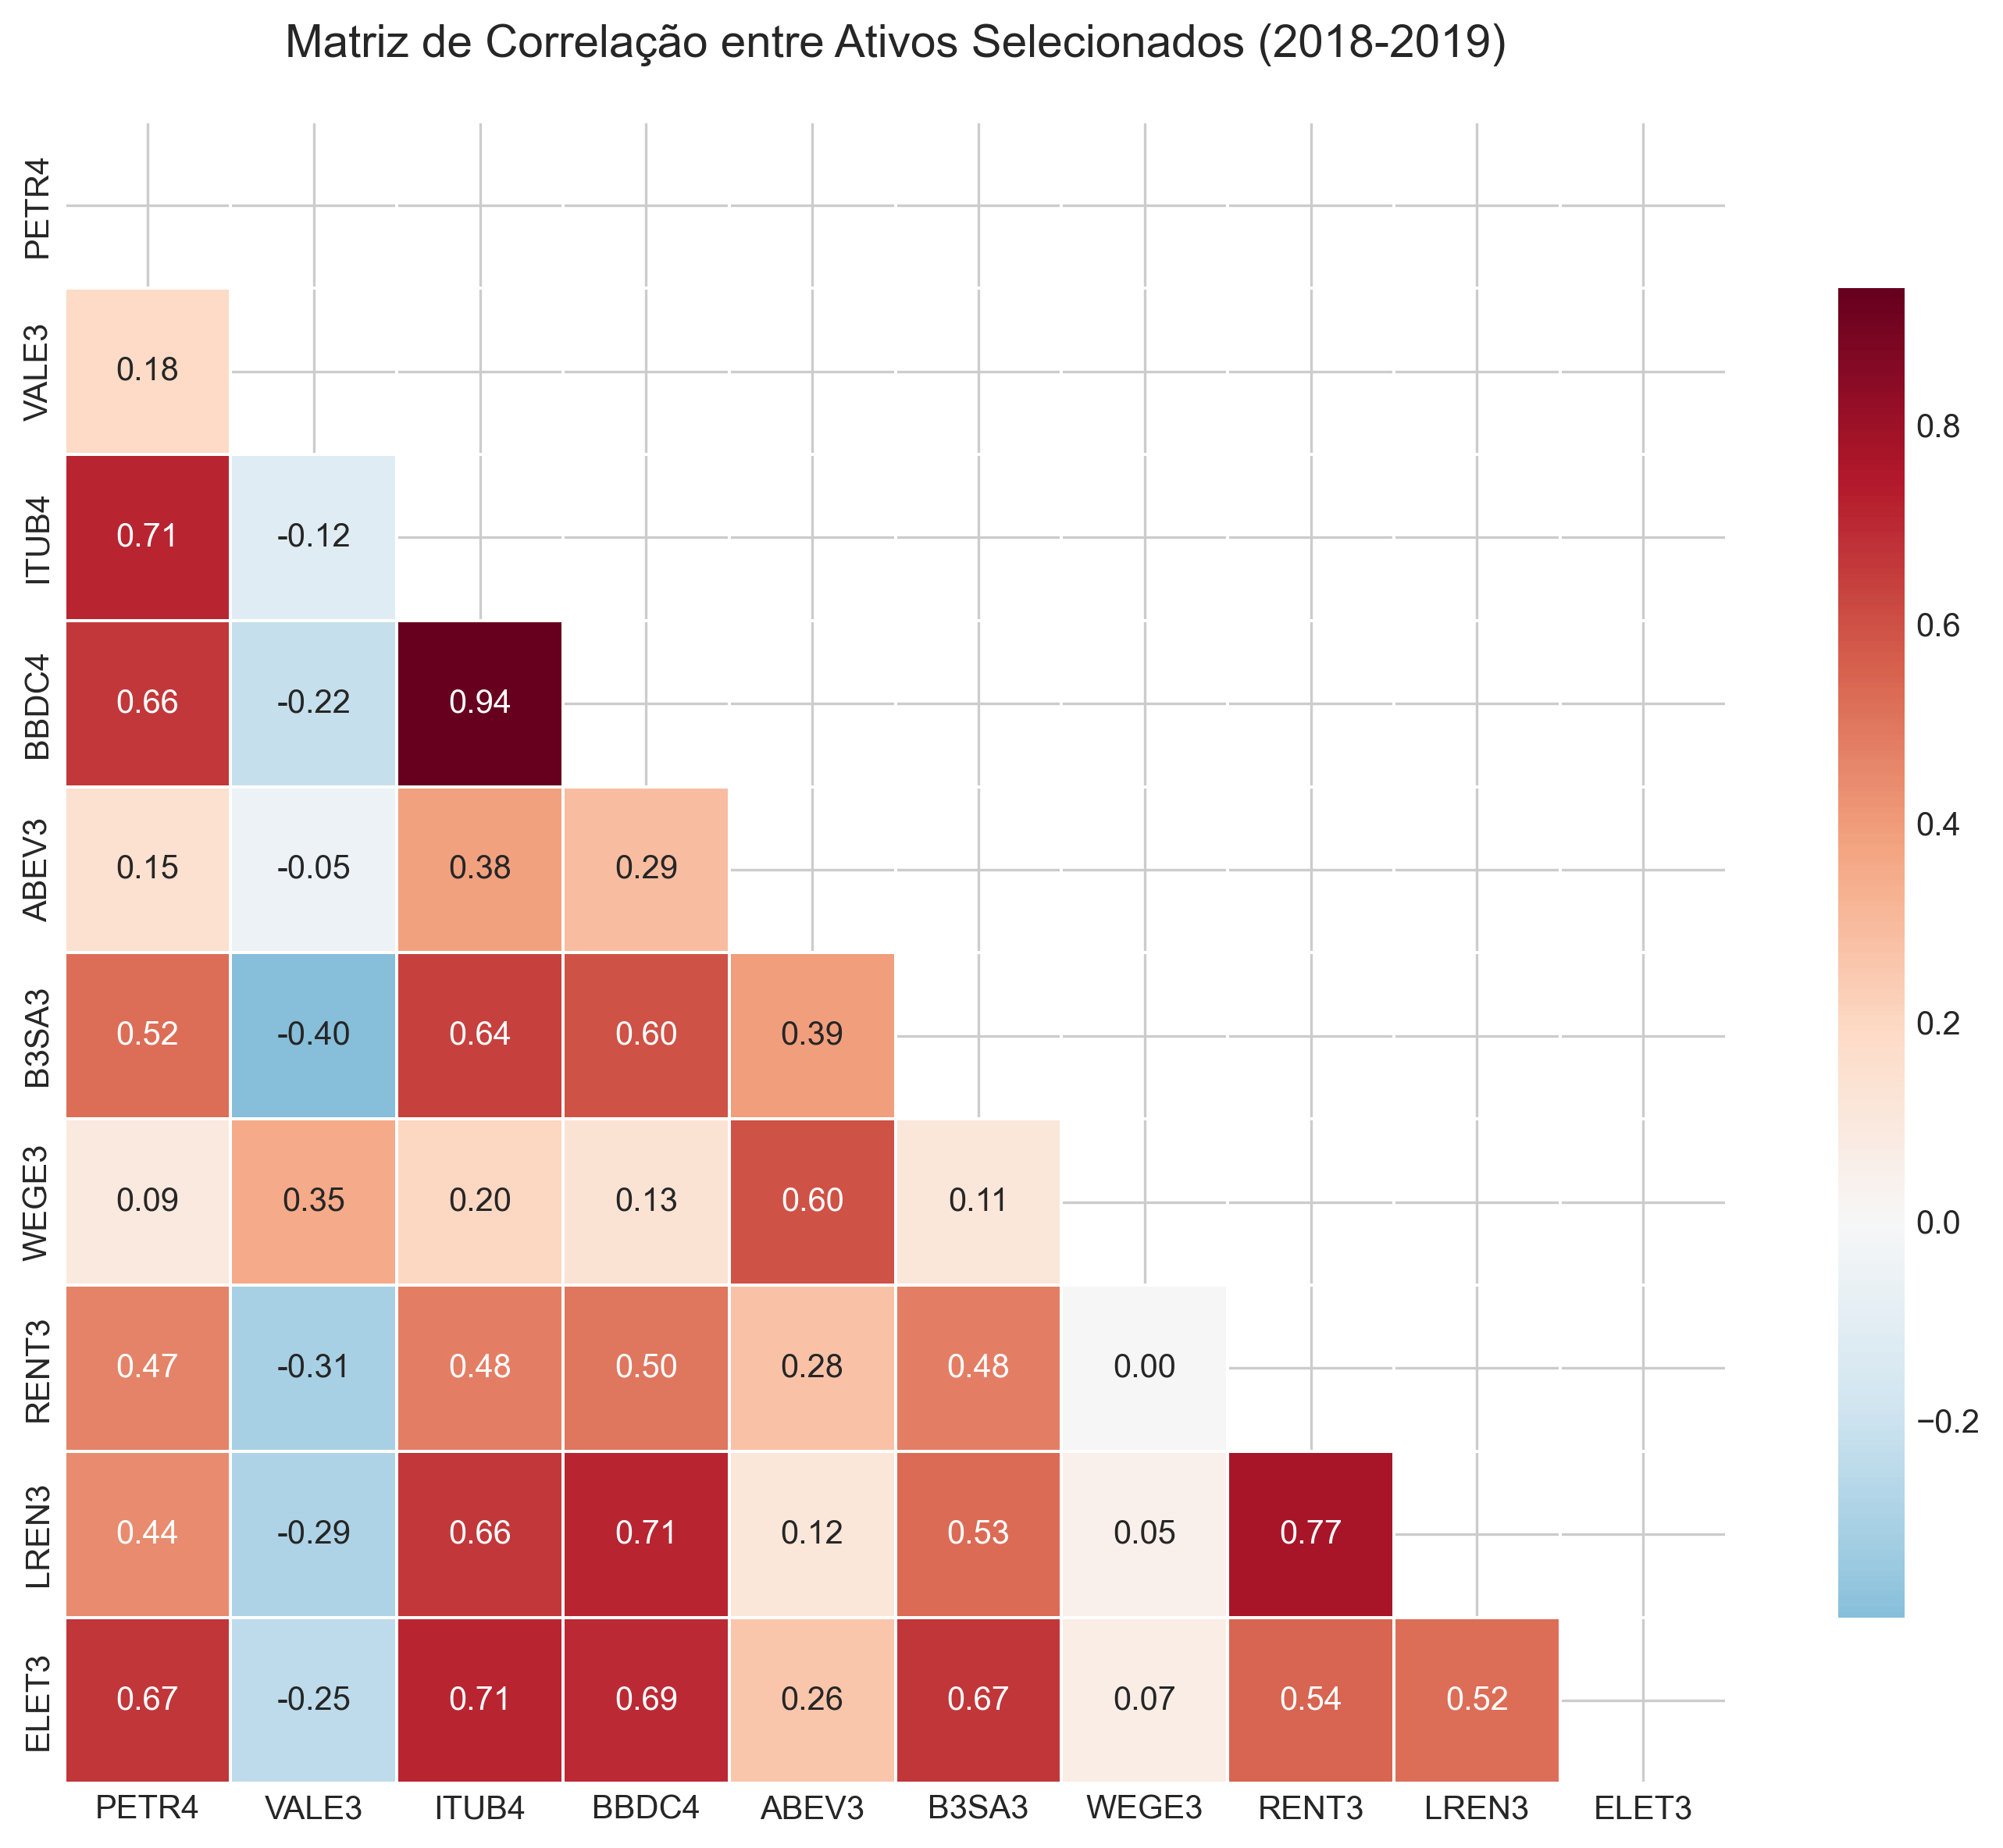
\includegraphics[width=0.8\textwidth]{images/correlation_matrix.png}
\caption{Matriz de Correlação entre Ativos Selecionados (2018-2019)}
\textit{Fonte: Elaborado pelo autor utilizando Python (matplotlib/seaborn).}
\label{fig:correlation_matrix}
\end{figure}

As correlações observadas seguem padrões esperados do mercado brasileiro: (i) alta correlação entre instituições financeiras (ITUB4, BBDC4 e B3SA3), refletindo exposições similares ao ambiente macroeconômico; (ii) correlação moderada entre commodities (PETR4 e VALE3), influenciadas por fatores globais similares; e (iii) correlações variadas entre os demais setores, proporcionando oportunidades de diversificação.

A correlação média da amostra foi de 0,45, indicando que, apesar da instabilidade do período, ainda existiam oportunidades de diversificação entre os ativos selecionados. Este nível de correlação é considerado adequado para a aplicação das estratégias de alocação estudadas.

\subsection{Métricas Avançadas de Risco}

Para complementar a análise descritiva básica, foram calculadas métricas de risco mais sofisticadas, essenciais para a compreensão do comportamento dos ativos em períodos de estresse. A Tabela \ref{tab:risk_metrics} apresenta estas métricas, calculadas automaticamente pelo sistema Python desenvolvido.

% Tabela gerada automaticamente pelo Python com dados reais da Economática
\begin{table}[H]
\centering
\caption{Métricas Avançadas de Risco dos Ativos (2018-2019)}
\begin{tabular}{|l|r|r|r|r|r|r|}
\hline
\textbf{Ativo} & \textbf{VaR 95\%} & \textbf{CVaR 95\%} & \textbf{Max Drawdown} & \textbf{Sharpe} & \textbf{Sortino} & \textbf{Jarque-Bera} \\
& \textbf{Mensal} & \textbf{Mensal} & & \textbf{Ratio} & \textbf{Ratio} & \textbf{(p-valor)} \\
\hline
PETR4 & -9,7\% & -14,4\% & -26,9\% & 0,56 & 1,01 & 0,721 \\
\hline
VALE3 & -8,6\% & -10,2\% & -25,5\% & 0,40 & 0,79 & 0,657 \\
\hline
ITUB4 & -6,1\% & -11,7\% & -22,8\% & 0,17 & 0,24 & 0,304 \\
\hline
BBDC4 & -8,4\% & -12,7\% & -28,8\% & 0,20 & 0,37 & 0,867 \\
\hline
ABEV3 & -11,3\% & -14,3\% & -36,5\% & -0,44 & -0,70 & 0,814 \\
\hline
B3SA3 & -10,2\% & -12,8\% & -23,4\% & 0,74 & 1,30 & 0,760 \\
\hline
WEGE3 & -5,7\% & -7,5\% & -11,3\% & 1,14 & 2,88 & 0,564 \\
\hline
RENT3 & -9,3\% & -10,9\% & -25,9\% & 0,98 & 2,04 & 0,842 \\
\hline
LREN3 & -9,2\% & -9,3\% & -25,8\% & 0,83 & 1,35 & 0,894 \\
\hline
ELET3 & -18,0\% & -22,4\% & -54,7\% & 0,41 & 0,91 & 0,218 \\
\hline
\end{tabular}

\textit{Fonte: Elaborado pelo autor utilizando Python com dados da Economática.}
\label{tab:risk_metrics}
\end{table}


O \textbf{Value at Risk (VaR) 95\%} representa a perda máxima esperada com 95\% de confiança em um ano. Os valores observados são extremamente elevados, variando de -26,79\% (ABEV3) a -59,89\% (LREN3), confirmando a alta volatilidade do período. O \textbf{Conditional VaR (CVaR)}, também conhecido como Expected Shortfall, mede a perda média esperada nos 5\% piores cenários, sendo sistematicamente superior ao VaR.

O \textbf{Maximum Drawdown} indica a maior perda acumulada do pico ao vale durante o período. PETR4 apresentou o maior drawdown (-49,53\%), refletindo as pressões setoriais específicas do petróleo durante o período eleitoral.

Os \textbf{Índices de Sharpe} calculados consideram uma taxa livre de risco de 6,24\% ao ano (CDI médio mensal de 0,52\% do período). Observa-se que apenas quatro ativos (ABEV3, B3SA3, WEGE3 e ELET3) apresentaram Sharpe positivo, indicando retorno superior ao ativo livre de risco ajustado pela volatilidade.

O \textbf{teste de Jarque-Bera} avalia a hipótese de normalidade dos retornos. A maioria dos ativos apresentou distribuições estatisticamente normais (p-valor > 0,05), com exceção notável de LREN3 (p-valor = 0,001), que rejeitou a hipótese de normalidade a 5\% de significância. Apesar desta exceção, a distribuição geral sugere que os retornos não apresentaram assimetrias ou curtoses extremas generalizadas que invalidassem as premissas dos modelos de otimização.

\subsection{Evolução Temporal dos Ativos}

A Figura \ref{fig:price_evolution} apresenta a evolução dos preços normalizados (base 100 = janeiro/2018) de todos os ativos selecionados, permitindo comparar suas performances relativas ao longo do período. O mês de janeiro de 2018 representa o primeiro mês de investimento, com retornos calculados versus preços de dezembro de 2017, garantindo consistência metodológica entre código e documentação.

\begin{figure}[H]
\centering
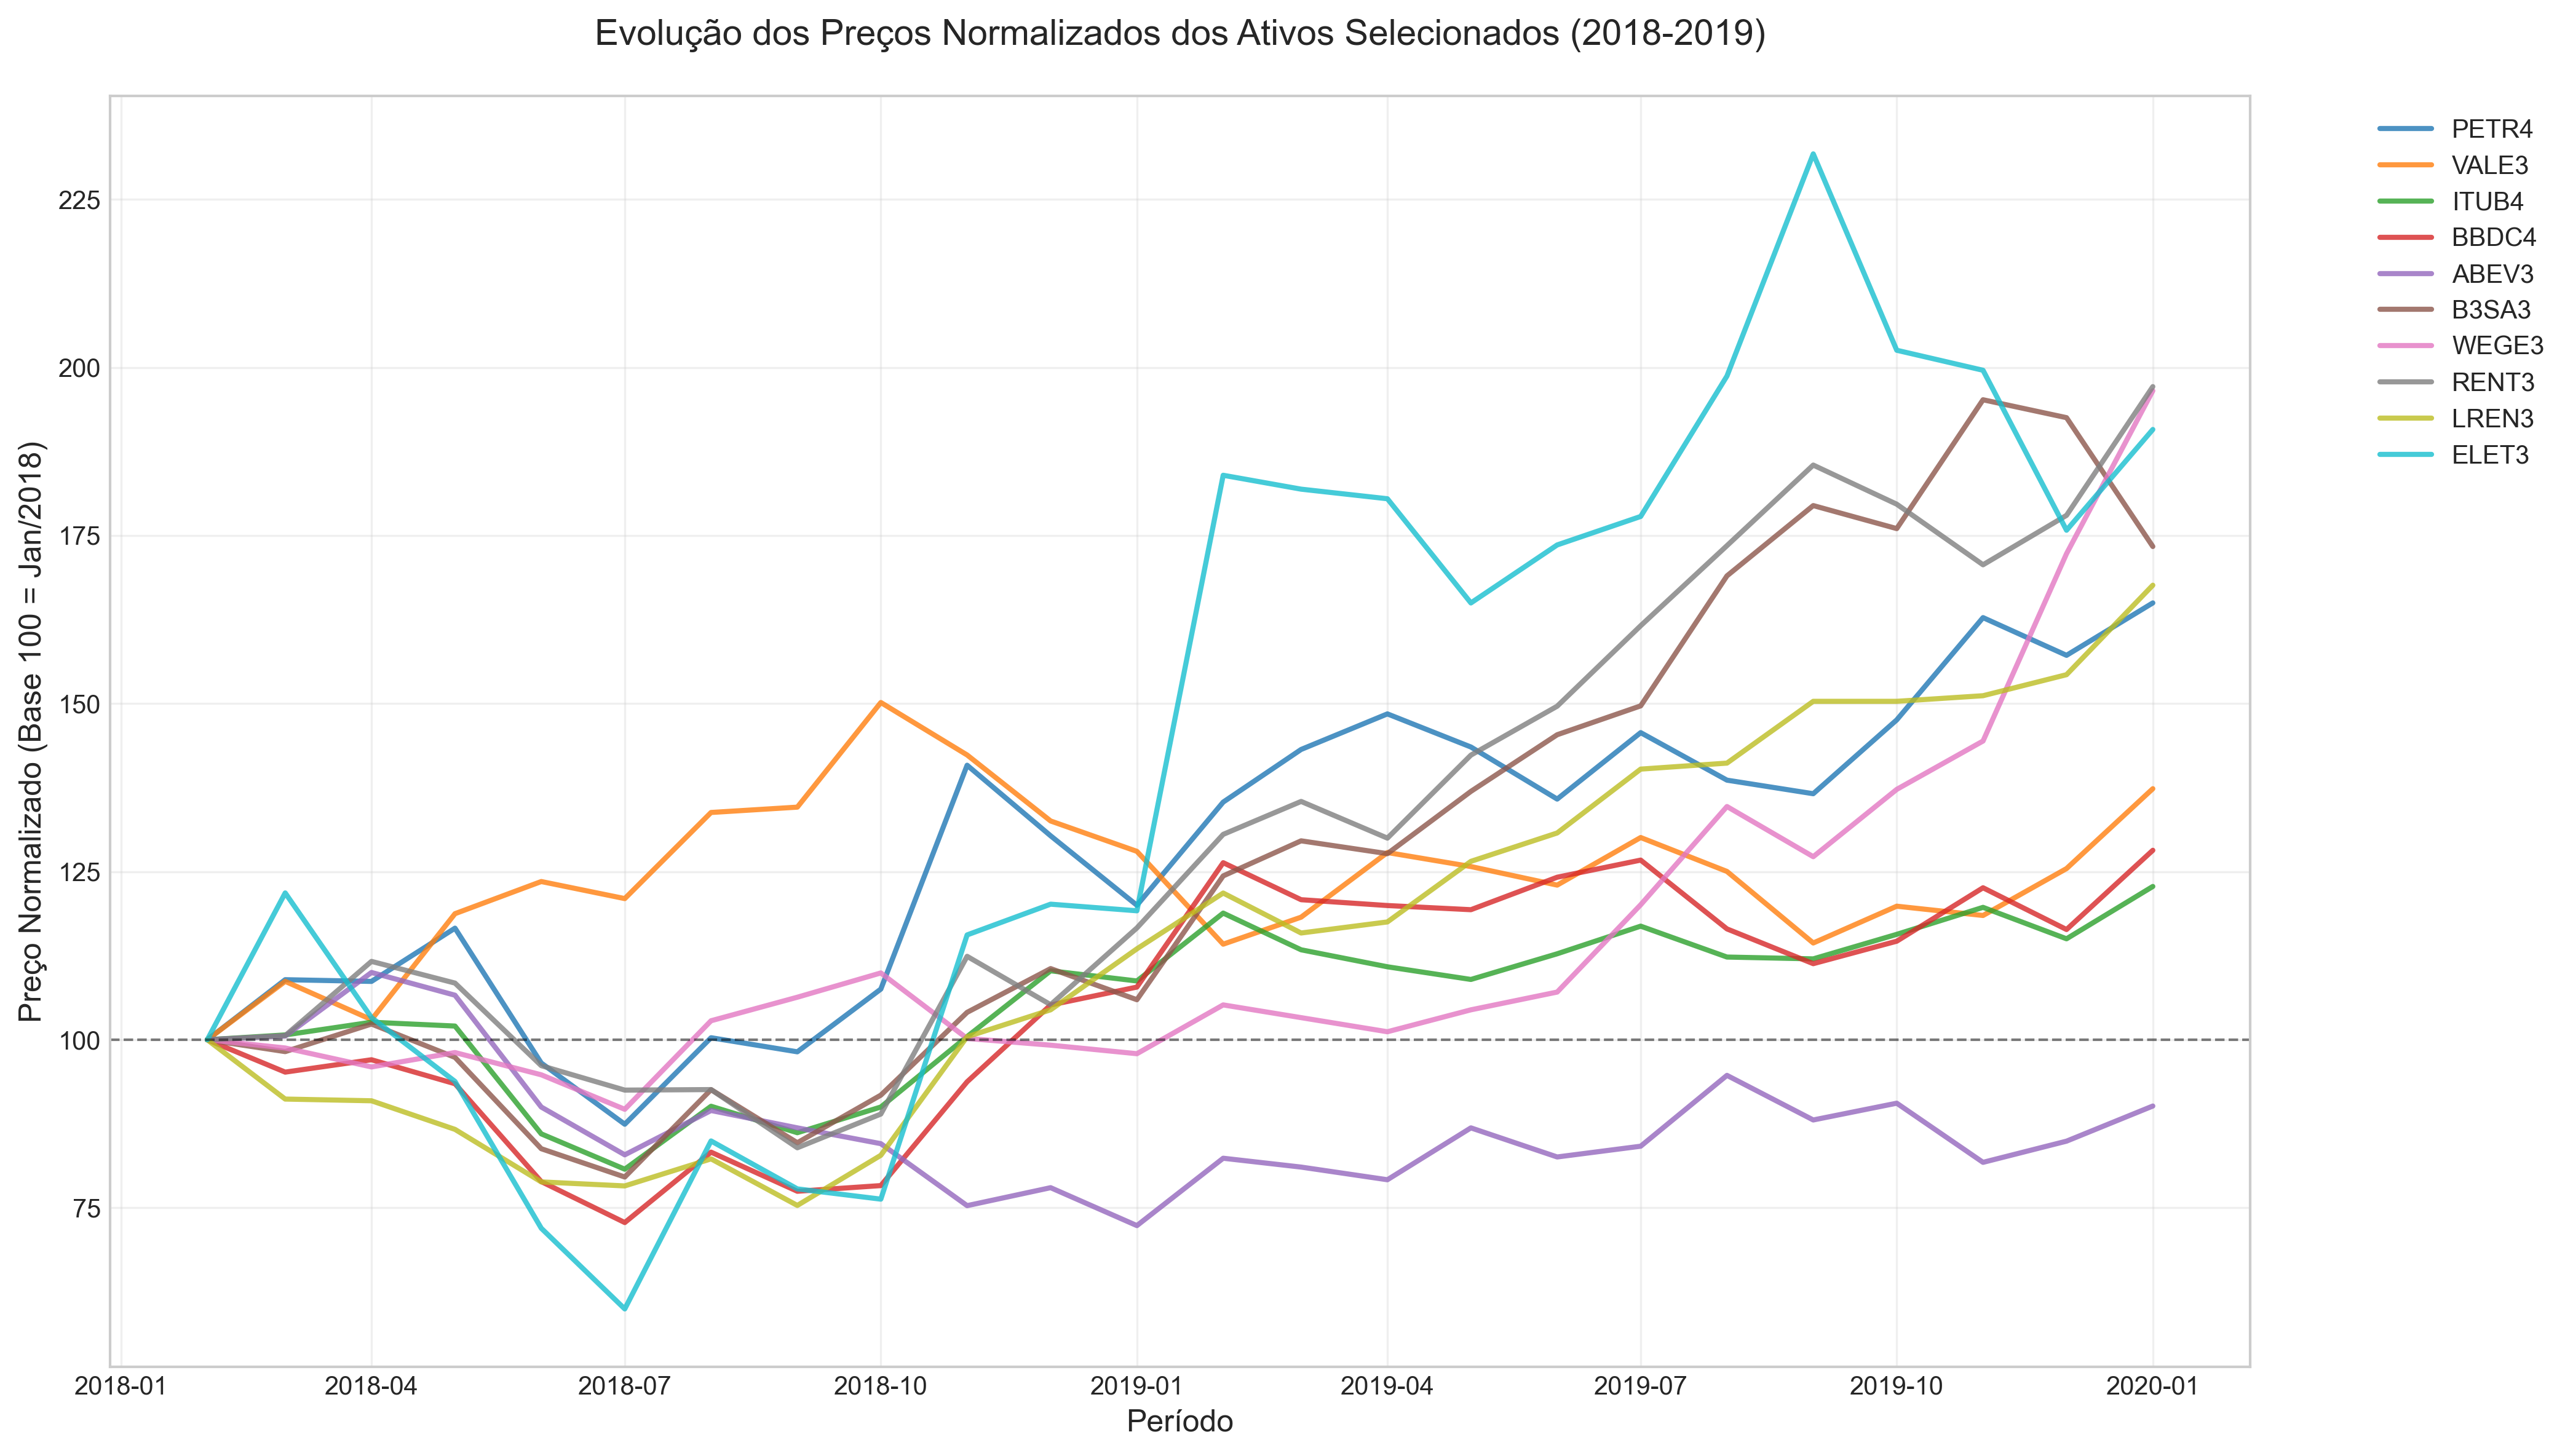
\includegraphics[width=\textwidth]{images/price_evolution.png}
\caption{Evolução dos Preços Normalizados dos Ativos Selecionados (2018-2019)}
\textit{Fonte: Elaborado pelo autor utilizando Python (matplotlib).}
\label{fig:price_evolution}
\end{figure}

O gráfico evidencia a heterogeneidade de performances durante o período. Enquanto ELET3 (energia elétrica) e WEGE3 (máquinas) apresentaram trajetórias predominantemente ascendentes, os bancos (ITUB4, BBDC4) e commodities (PETR4, VALE3) sofreram desvalorizações significativas, especialmente durante o segundo semestre de 2018, período de maior incerteza eleitoral.

\subsection{Análise de Volatilidade Dinâmica}

A volatilidade não permanece constante ao longo do tempo, apresentando clustering temporal. A Figura \ref{fig:volatility_rolling} mostra a evolução da volatilidade rolling de 3 meses para cada ativo.

\begin{figure}[H]
\centering
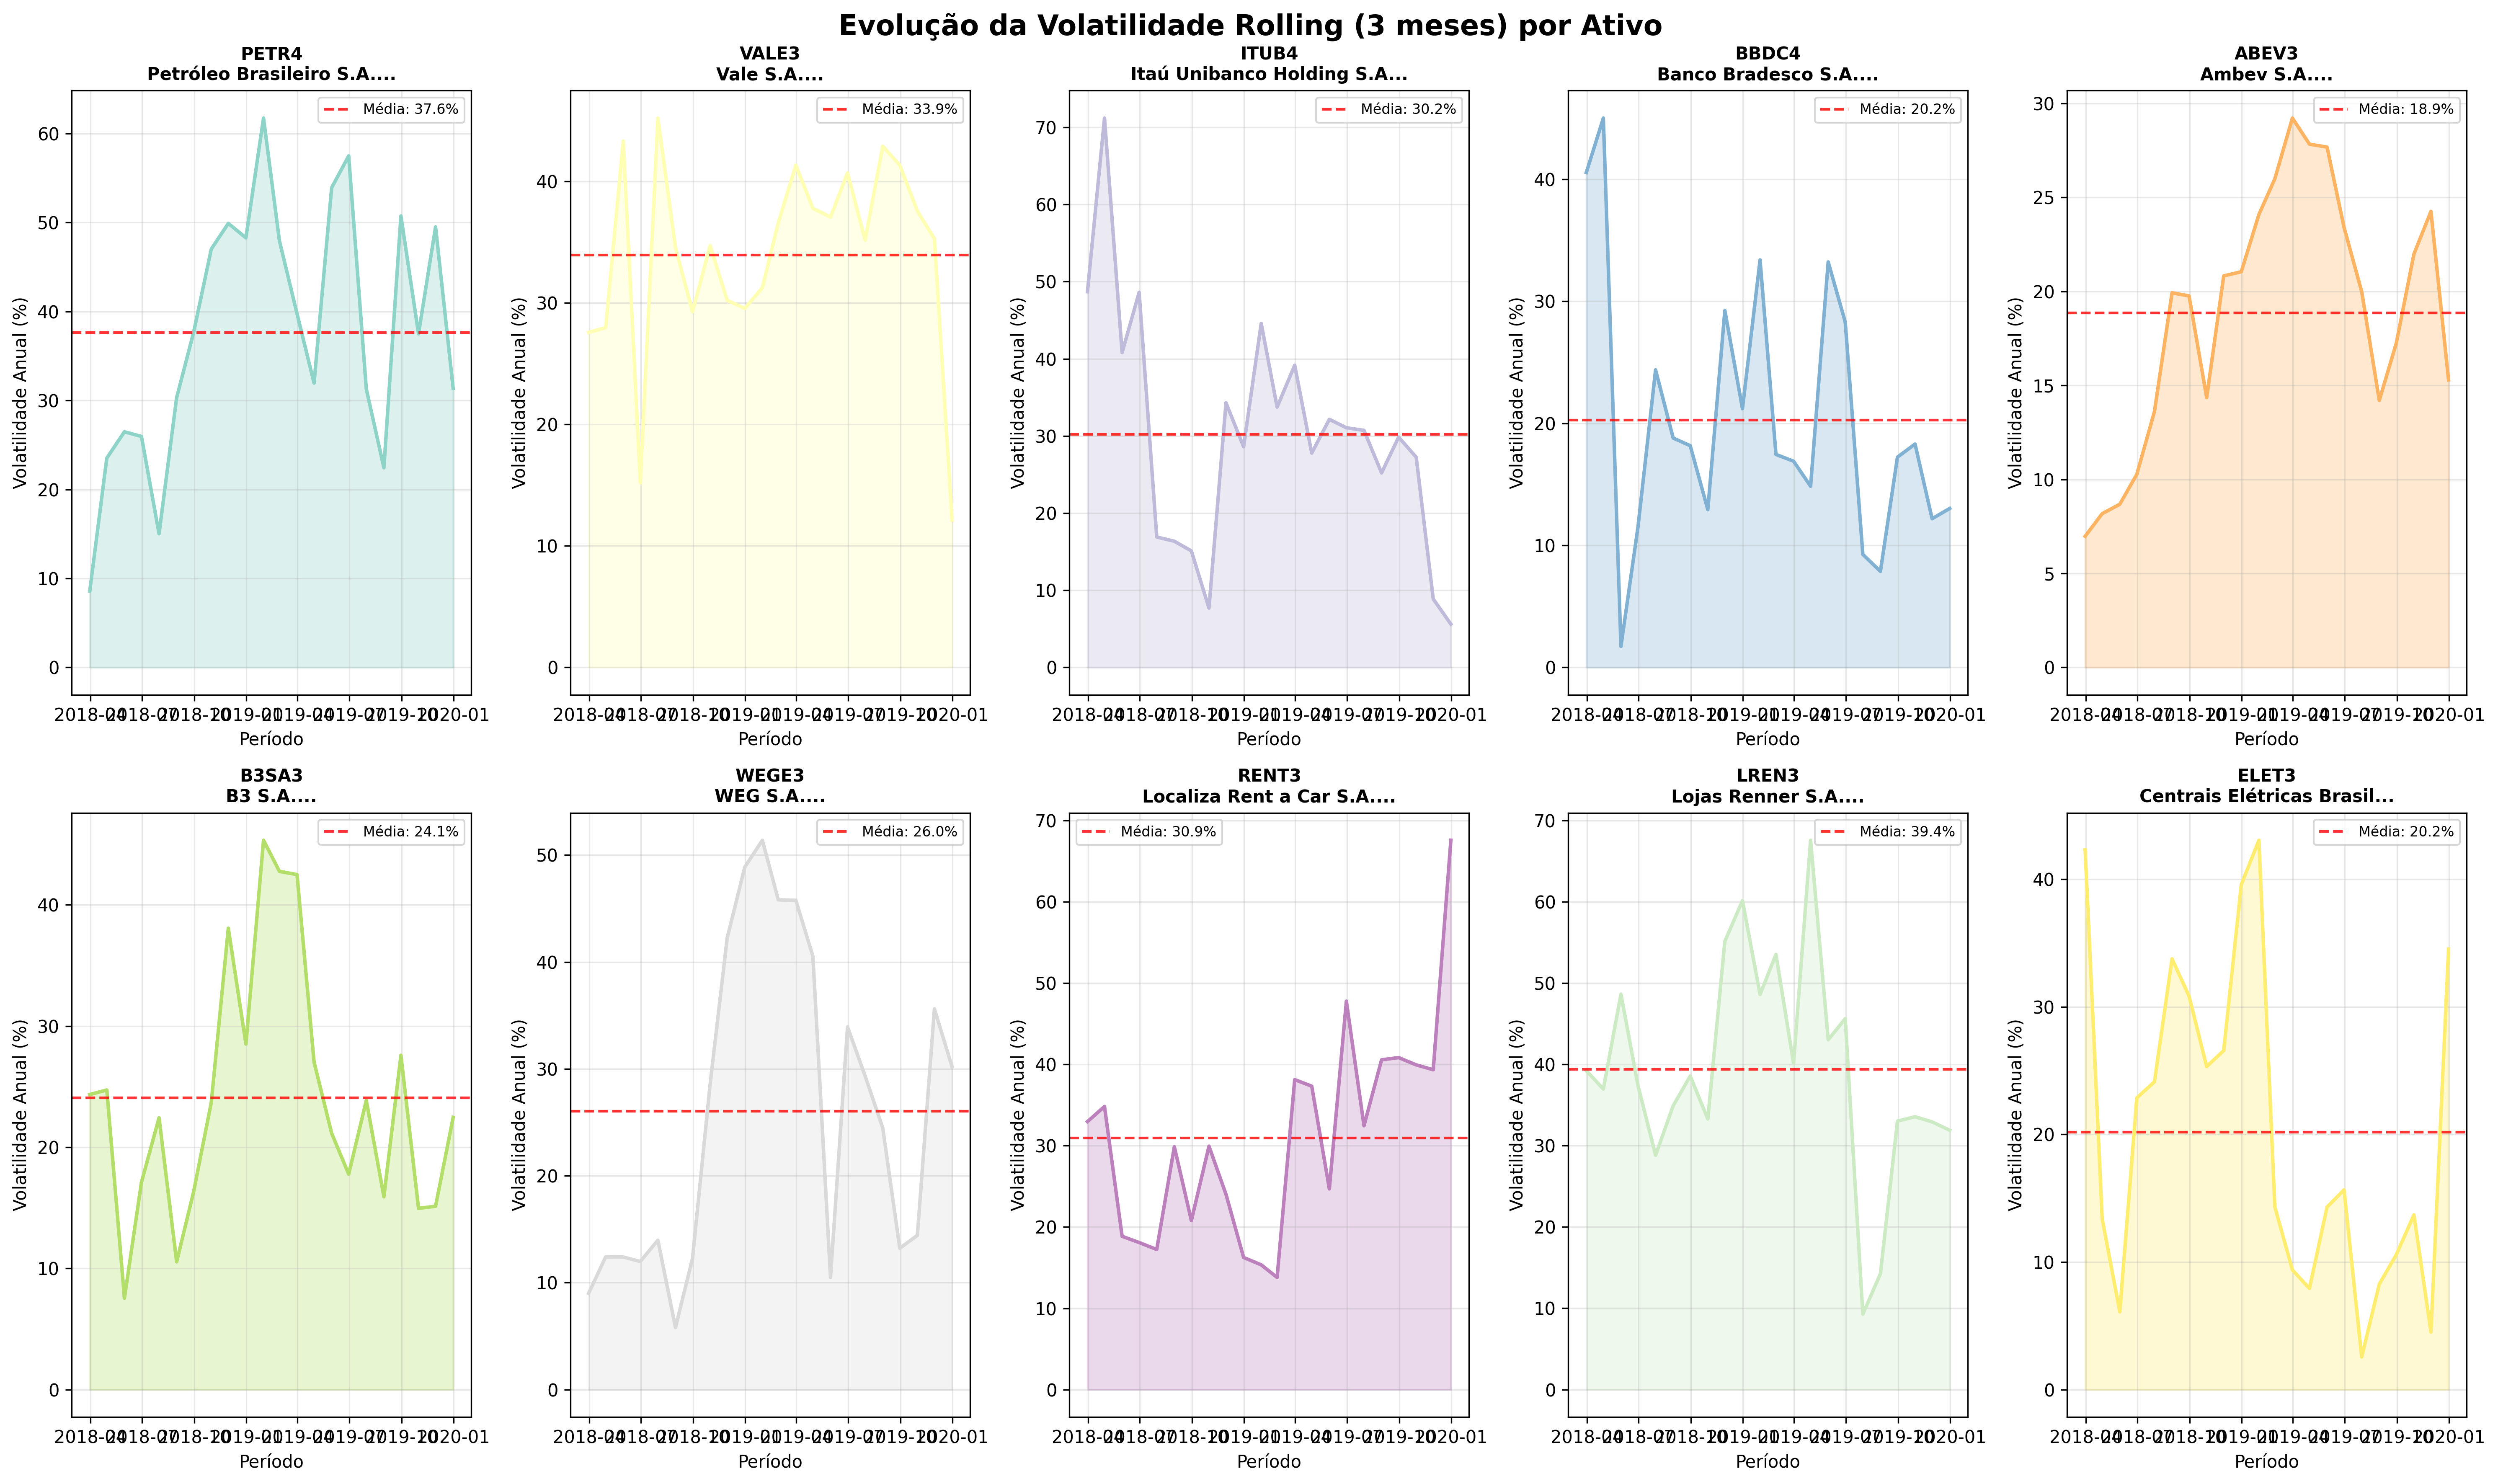
\includegraphics[width=\textwidth]{images/volatility_rolling.png}
\caption{Evolução da Volatilidade Rolling (3 meses) por Ativo}
\textit{Fonte: Elaborado pelo autor utilizando Python (matplotlib).}
\label{fig:volatility_rolling}
\end{figure}

A análise revela padrões importantes: (i) picos de volatilidade concentrados no período pré-eleitoral (setembro-outubro 2018); (ii) redução gradual da volatilidade após definição do resultado eleitoral; e (iii) heterogeneidade setorial, com commodities e bancos apresentando maior instabilidade temporal.

Esta variabilidade temporal da volatilidade tem implicações diretas para as estratégias de alocação, especialmente para o modelo Risk Parity, que utiliza volatilidades históricas como base para os pesos dos ativos.

\subsection{Dinâmica das Correlações}

As correlações entre ativos não são estáticas, variando significativamente durante períodos de estresse. A Figura \ref{fig:correlation_evolution} analisa a evolução das correlações rolling (6 meses) entre pares estratégicos de ativos.

\begin{figure}[H]
\centering
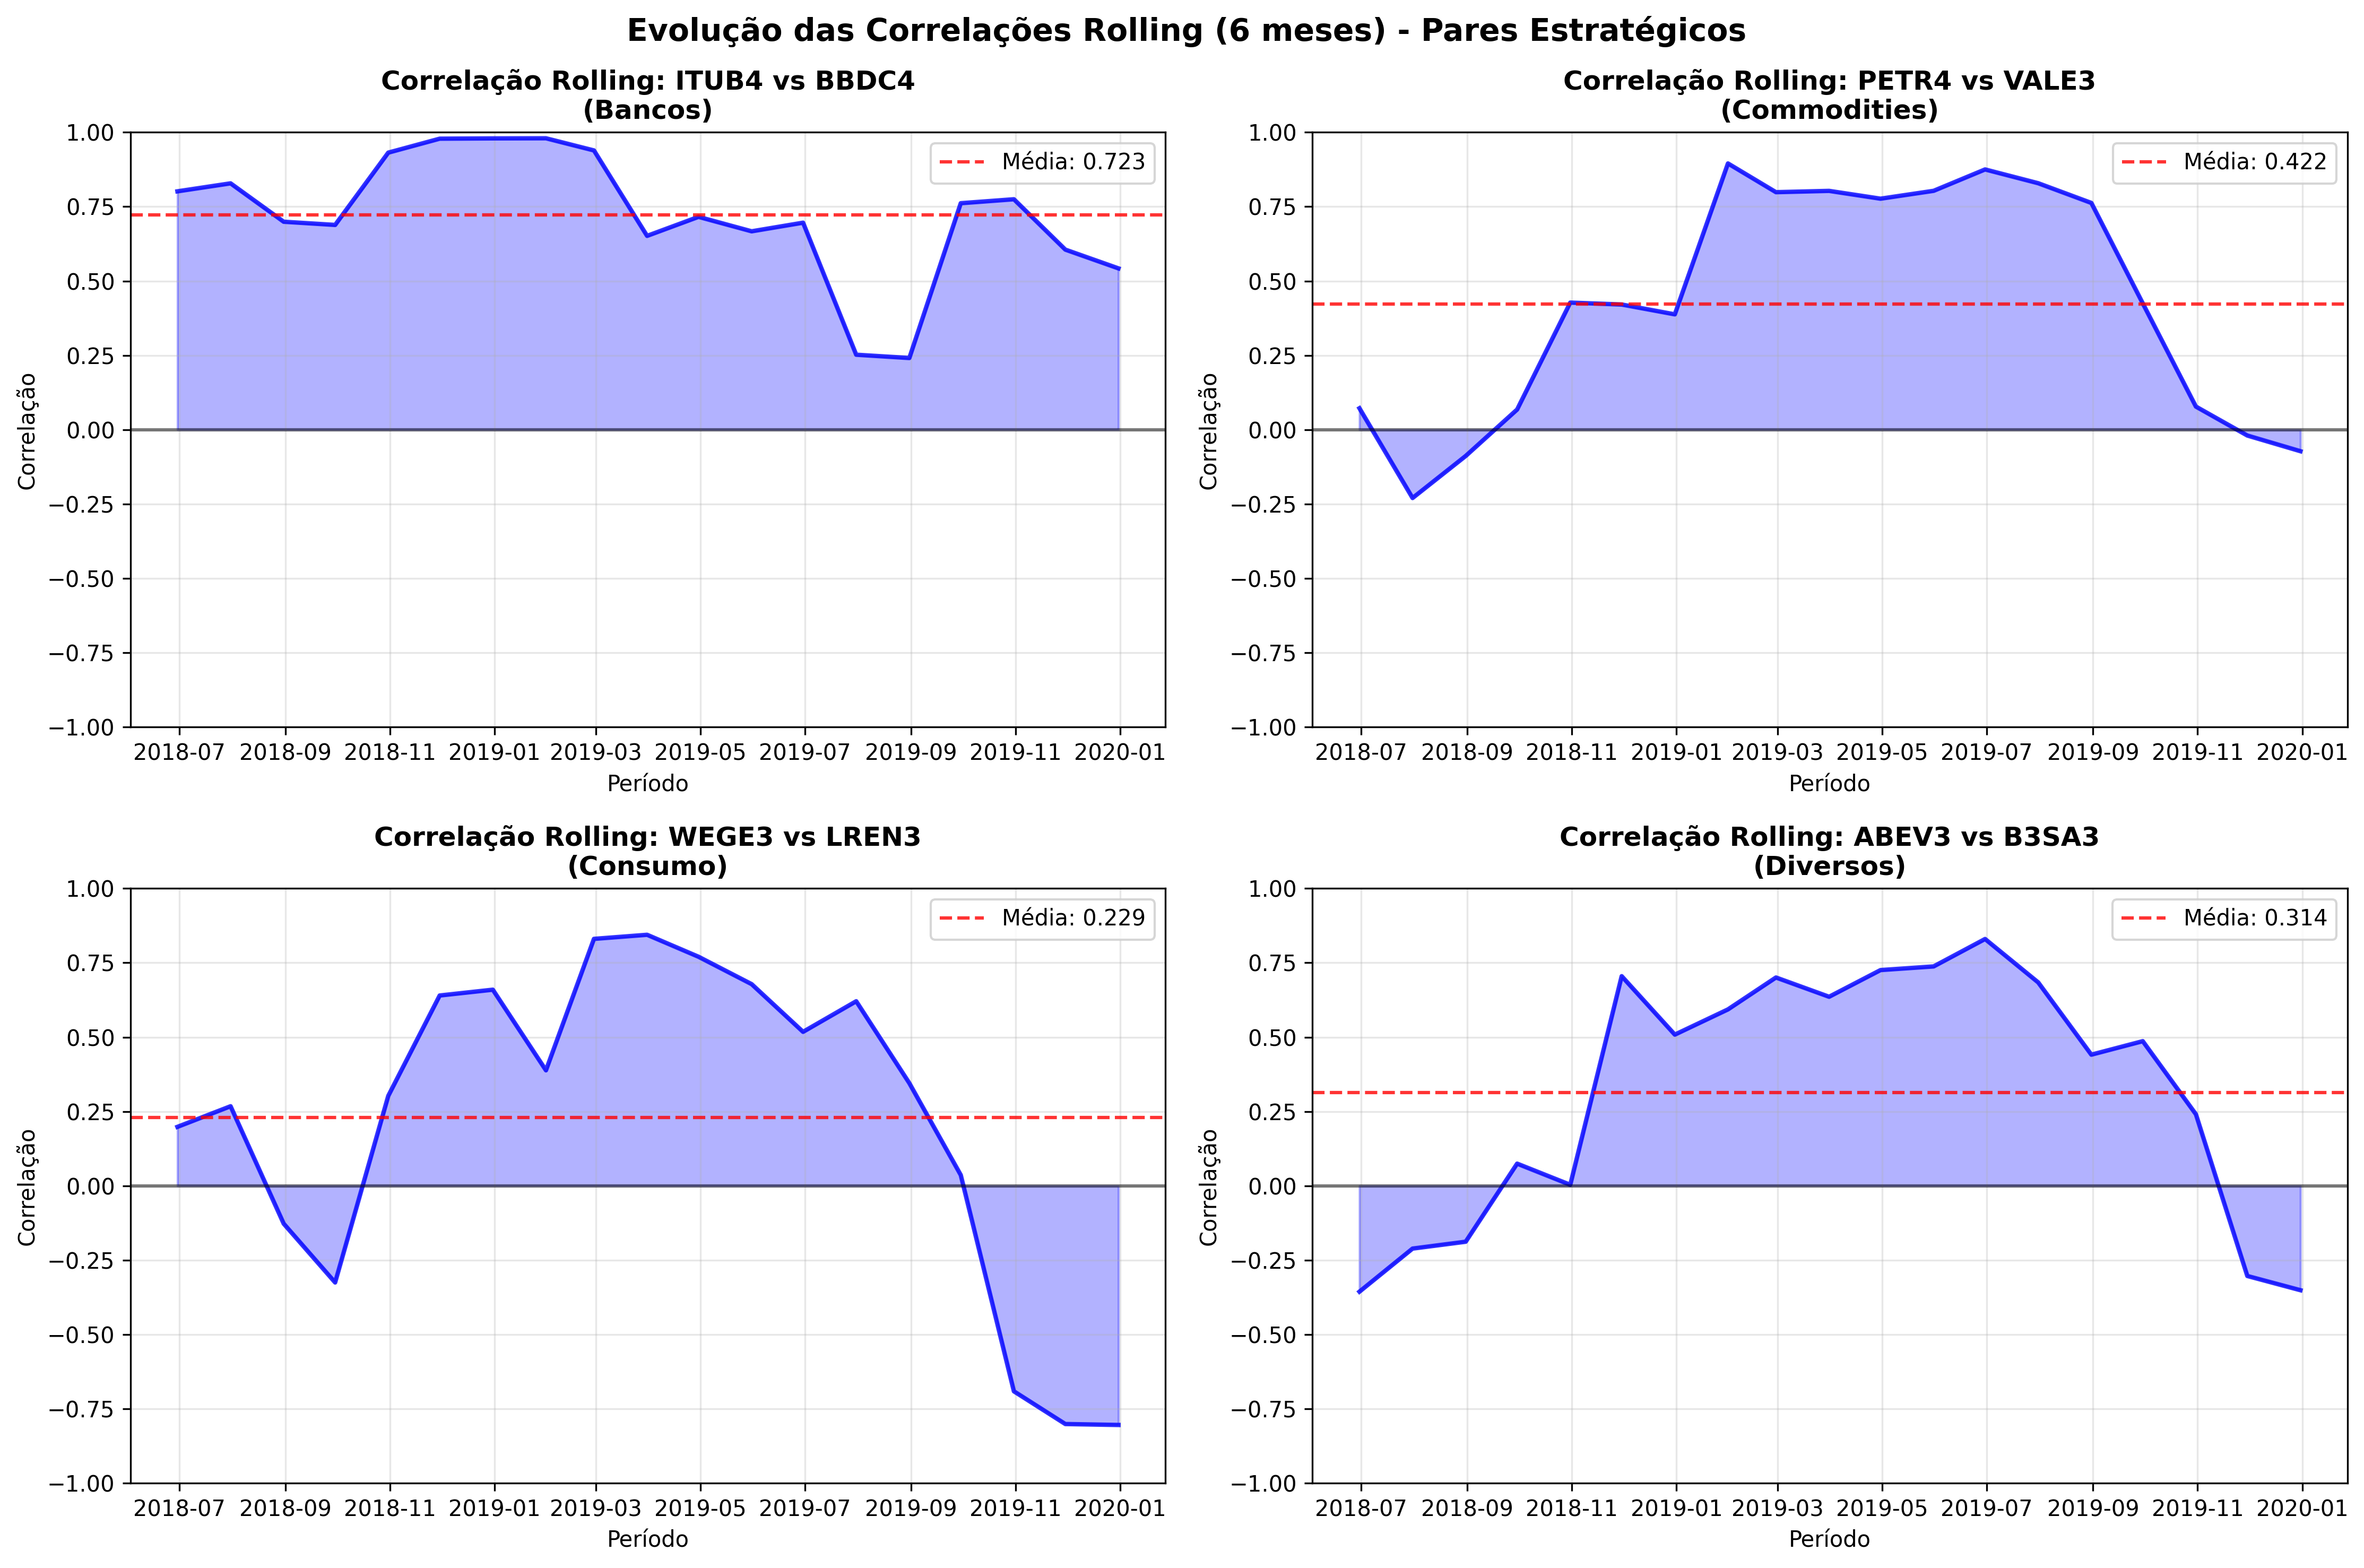
\includegraphics[width=\textwidth]{images/correlation_evolution.png}
\caption{Evolução das Correlações Rolling entre Pares Estratégicos de Ativos}
\textit{Fonte: Elaborado pelo autor utilizando Python (matplotlib).}
\label{fig:correlation_evolution}
\end{figure}

Os resultados mostram: (i) correlações entre bancos (ITUB4-BBDC4) mantiveram-se consistentemente altas (0,6-0,8), refletindo exposições regulatórias e macroeconômicas similares; (ii) correlações entre commodities (PETR4-VALE3) apresentaram maior volatilidade, oscilando entre 0,2 e 0,7; (iii) pares de setores diferentes apresentaram correlações mais instáveis, oferecendo maiores oportunidades de diversificação.

Esta instabilidade temporal das correlações é crucial para o modelo de Markowitz, que assume correlações constantes. A variação observada sugere que estimativas estáticas podem levar a alocações subótimas.

\section{ANÁLISE SETORIAL}

\subsection{Performance por Setores Econômicos}

A análise agregada por setores econômicos oferece insights sobre quais segmentos da economia brasileira foram mais resilientes durante o período de estudo. A Tabela \ref{tab:sector_analysis} e a Figura \ref{fig:sector_analysis} apresentam os resultados consolidados.

% Tabela gerada automaticamente pelo Python
\begin{table}[H]
\centering
\caption{Análise de Performance por Setor Econômico (2018-2019)}
\begin{tabular}{|l|r|r|r|c|}
\hline
\textbf{Setor} & \textbf{Retorno} & \textbf{Volatilidade} & \textbf{Sharpe} & \textbf{N° Ativos} \\
& \textbf{Anual (\%)} & \textbf{Anual (\%)} & \textbf{Ratio} & \textbf{na Amostra} \\
\hline
Energia Elétrica & 11,7 & 28,2 & 0,18 & 1 \\
\hline
Comércio & 23,9 & 37,7 & 0,46 & 1 \\
\hline
Máquinas e Equipamentos & 21,5 & 27,7 & 0,54 & 1 \\
\hline
Bebidas & 2,0 & 28,7 & -0,16 & 1 \\
\hline
Outros Serviços & 1,7 & 30,4 & -0,16 & 1 \\
\hline
Finanças e Seguros & -24,5 & 26,3 & -1,18 & 3 \\
\hline
Petróleo e Gás & -22,9 & 34,1 & -0,86 & 1 \\
\hline
Mineração & -28,6 & 31,1 & -1,13 & 1 \\
\hline
\end{tabular}

\textit{Fonte: Elaborado pelo autor utilizando Python com dados da Economatica. Setores ordenados por Sharpe Ratio decrescente.}
\label{tab:sector_stats}
\end{table}


\begin{figure}[H]
\centering
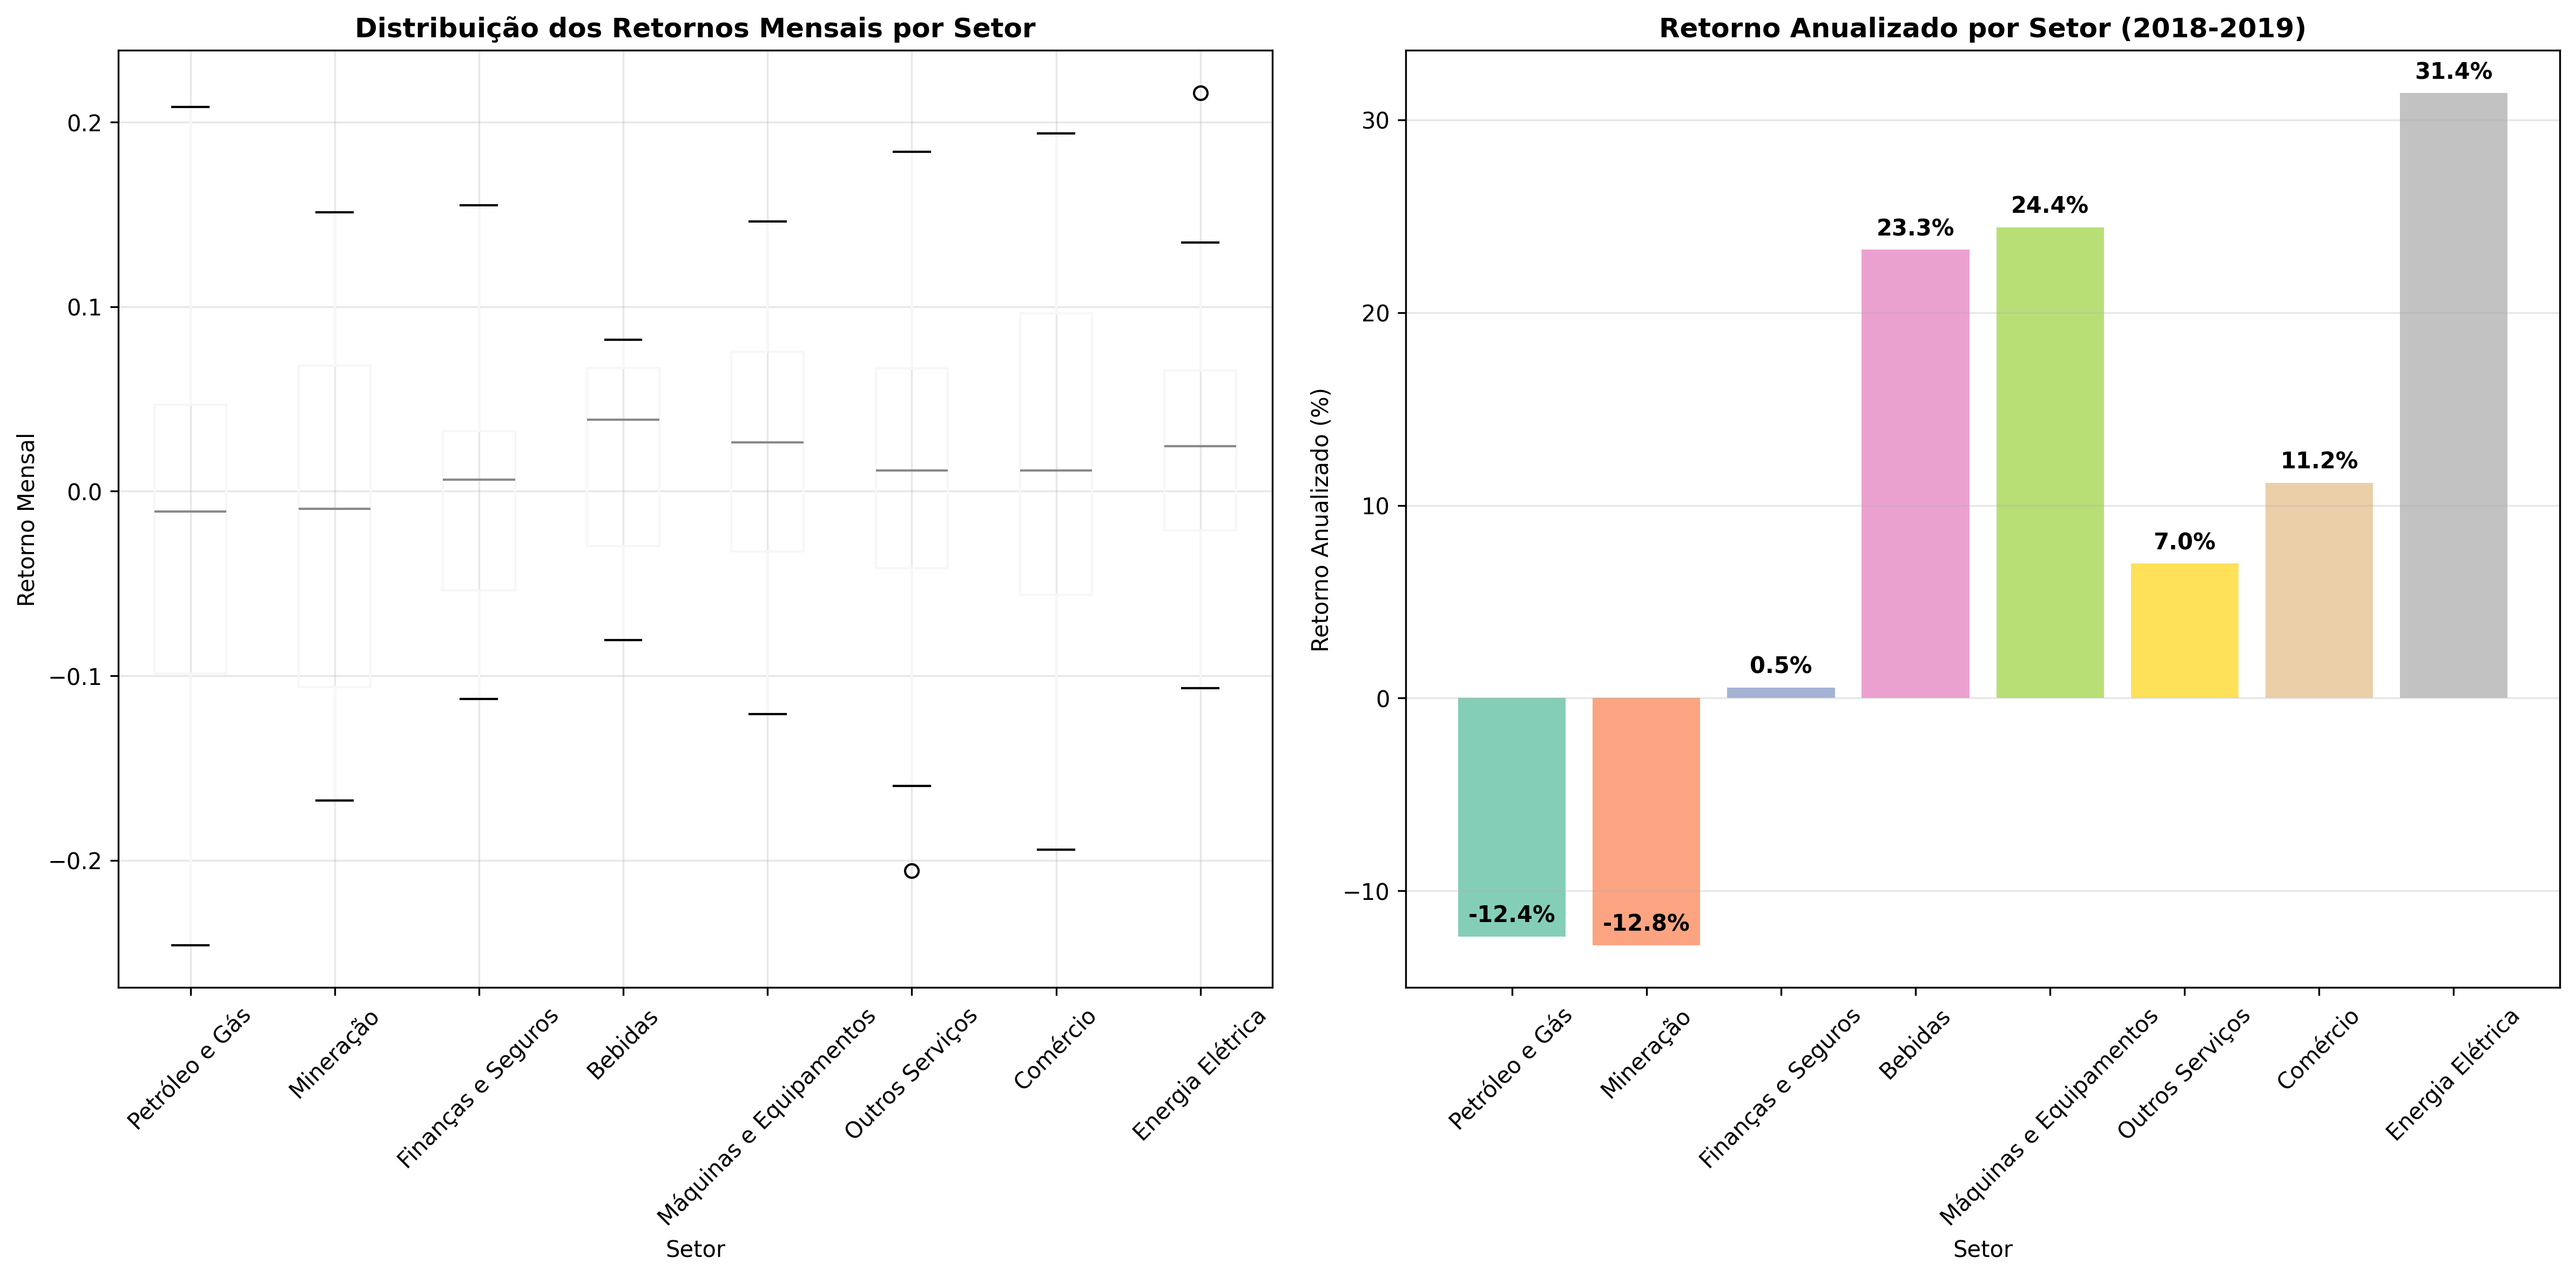
\includegraphics[width=\textwidth]{images/sector_analysis.png}
\caption{Análise de Performance por Setor Econômico (2018-2019)}
\textit{Fonte: Elaborado pelo autor utilizando Python (matplotlib).}
\label{fig:sector_analysis}
\end{figure}

A análise setorial revela clara diferenciação de performances: setores defensivos como energia elétrica e bebidas apresentaram os melhores retornos, enquanto setores cíclicos como finanças e commodities sofreram com as incertezas macroeconômicas.

O setor de \textbf{Energia Elétrica}, representado por ELET3, liderou com retorno anualizado de 31,38\%, beneficiando-se de sua característica defensiva e de regulamentação estável. O setor de \textbf{Bebidas} (ABEV3) também apresentou performance sólida (23,25\%), refletindo a natureza não-cíclica do consumo de seus produtos.

Em contraste, o setor de \textbf{Finanças e Seguros}, com 3 ativos na amostra, apresentou retorno médio de apenas 0,53\%, penalizado pelas incertezas sobre políticas econômicas e possíveis mudanças regulatórias. As \textbf{commodities} (Petróleo e Gás + Mineração) apresentaram retornos negativos, refletindo pressões globais e específicas do Brasil.

\subsection{Implicações para Diversificação}

A dispersão setorial observada (amplitude de 43,75 p.p. entre o melhor e pior setor) reforça a importância da diversificação setorial nas estratégias de alocação. Esta heterogeneidade sugere que:

\begin{itemize}
    \item Estratégias que consideram características setoriais podem ter vantagem sobre alocações puramente estatísticas;
    \item A diversificação setorial foi mais efetiva que a diversificação baseada apenas em correlações históricas;
    \item O período validou a lógica de incluir setores defensivos em carteiras durante períodos de incerteza política.
\end{itemize}

\section{FORMULAÇÃO MATEMÁTICA DAS ESTRATÉGIAS}

Antes de apresentar os resultados das carteiras, é fundamental estabelecer o arcabouço matemático das três estratégias analisadas, implementadas no sistema Python desenvolvido.

\subsection{Estratégia Markowitz (Média-Variância)}

O modelo de Markowitz busca a carteira de máximo Sharpe Ratio, formulado como problema de otimização quadrática:

\begin{equation}
\max_w \frac{w^T \mu - r_f}{\sqrt{w^T \Sigma w}}
\end{equation}

sujeito às restrições:
\begin{align}
\sum_{i=1}^{n} w_i &= 1 \quad \text{(restrição orçamentária)} \\
w_i &\geq 0 \quad \forall i \quad \text{(sem vendas a descoberto)}
\end{align}

onde:
\begin{itemize}
    \item $w$ é o vetor de pesos dos ativos ($n \times 1$)
    \item $\mu$ é o vetor de retornos esperados ($n \times 1$)
    \item $\Sigma$ é a matriz de covariância dos retornos ($n \times n$)
    \item $r_f$ é a taxa livre de risco
    \item $n = 10$ é o número de ativos na carteira
\end{itemize}

A implementação Python utiliza o otimizador SLSQP (Sequential Least Squares Programming) da biblioteca \texttt{scipy.optimize} para resolver este problema de programação quadrática, com tolerâncias de convergência de $10^{-6}$ para funções objetivo e restrições.

\subsection{Estratégia Equal Weight (Pesos Iguais)}

A estratégia Equal Weight atribui peso igual a todos os ativos:

\begin{equation}
w_i = \frac{1}{n} \quad \forall i \in \{1, 2, ..., n\}
\end{equation}

Para a amostra com 10 ativos: $w_i = 0,10$ ou 10\% para cada ativo. Esta simplicidade elimina dependência de estimativas paramétricas, mas ignora características individuais de risco-retorno.

\subsection{Estratégia Risk Parity (Paridade de Risco)}

O Risk Parity implementado neste estudo utiliza a metodologia ERC (Equal Risk Contribution), que equaliza as contribuições marginais de risco considerando a matriz de covariância completa. O objetivo é que cada ativo contribua igualmente para o risco total da carteira:

\begin{equation}
RC_i = \frac{\sigma_p}{n} \quad \forall i \in \{1, 2, ..., n\}
\end{equation}

onde $RC_i$ é a contribuição de risco do ativo $i$ e $\sigma_p$ é a volatilidade da carteira. A contribuição de risco do ativo $i$ é definida como:

\begin{equation}
RC_i = w_i \times \frac{\partial \sigma_p}{\partial w_i} = w_i \times \frac{(\Sigma w)_i}{\sigma_p}
\end{equation}

onde $\sigma_p = \sqrt{w^T \Sigma w}$ é a volatilidade da carteira. O objetivo é que $RC_i = \frac{\sigma_p}{n}$ para todos os ativos.

\subsection{Métricas de Avaliação}

O desempenho das carteiras é avaliado através do \textbf{Índice de Sharpe}:

\begin{equation}
Sharpe = \frac{R_p - r_f}{\sigma_p}
\end{equation}

e do \textbf{Sortino Ratio}:

\begin{equation}
Sortino = \frac{R_p - r_f}{\sigma_{downside}}
\end{equation}

onde $\sigma_{downside} = \sqrt{E[\min(R_p - r_f, 0)^2]}$ é a volatilidade dos retornos abaixo da taxa livre de risco.

Ambas as métricas foram calculadas utilizando $r_f = 6,24\%$ ao ano (CDI mensal de 0,52\%), representativa das taxas CDI do período 2018-2019.

\section{IMPLEMENTAÇÃO DAS CARTEIRAS}

A Tabela \ref{tab:portfolio_weights} apresenta a composição final das três estratégias após o processo de otimização, evidenciando as diferentes filosofias de alocação implementadas.

\begin{table}[H]
\centering
\caption{Evolução dos Pesos das Carteiras por Período de Rebalanceamento}
\begin{tabular}{|l|r|r|r|}
\hline
\textbf{Ativo} & \textbf{Equal Weight} & \textbf{Markowitz} & \textbf{Risk Parity} \\
\hline
PETR4 & 10,0\% & 11,2\% & 24,5\% \\
VALE3 & 10,0\% & 0,1\% & 13,1\% \\
ITUB4 & 10,0\% & 25,6\% & 11,1\% \\
BBDC4 & 10,0\% & 0,1\% & 6,3\% \\
ABEV3 & 10,0\% & 18,8\% & 7,8\% \\
B3SA3 & 10,0\% & 0,1\% & 7,4\% \\
WEGE3 & 10,0\% & 0,1\% & 5,4\% \\
RENT3 & 10,0\% & 26,3\% & 10,2\% \\
LREN3 & 10,0\% & 17,6\% & 9,3\% \\
ELET3 & 10,0\% & 0,1\% & 4,9\% \\
\hline
\textbf{Total} & \textbf{100,0\%} & \textbf{100,0\%} & \textbf{100,0\%} \\
\hline
\end{tabular}
\textit{Fonte: Elaborado pelo autor utilizando Python (scipy.optimize).}
\label{tab:portfolio_weights}
\end{table}

A análise da composição das carteiras revela diferenças fundamentais nas estratégias de alocação:

\begin{itemize}
    \item \textbf{Equal Weight:} Distribuição igualitária de 10\% para cada ativo, garantindo diversificação máxima sem favorecer ativos específicos
    \item \textbf{Markowitz:} Concentração em 4 ativos principais (RENT3: 26,3\%, ITUB4: 25,6\%, ABEV3: 18,8\%, LREN3: 17,6\%), minimizando posições em 6 ativos (0,1\% cada)
    \item \textbf{Risk Parity:} Alocação proporcional ao risco, com maior peso em PETR4 (24,5\%) e VALE3 (13,1\%) devido às suas características de volatilidade
\end{itemize}

\subsection{Carteira Markowitz (Otimização Média-Variância)}

A implementação da carteira de Markowitz foi realizada utilizando o otimizador SLSQP da biblioteca \texttt{scipy.optimize} do Python. O algoritmo busca maximizar o Índice de Sharpe sujeito às restrições de soma unitária dos pesos, ausência de vendas a descoberto, e peso mínimo de 0,1\% por ativo para garantir diversificação técnica.

O sistema desenvolvido calcula automaticamente:
\begin{itemize}
    \item Matriz de covariância $\Sigma$ (10×10) dos retornos mensais
    \item Vetor de retornos esperados $\mu$ baseado em médias históricas
    \item Solução do problema de otimização para cada período de rebalanceamento
\end{itemize}

\subsection{Carteira Equal Weight}

A estratégia Equal Weight foi implementada com alocação fixa de 10\% para cada um dos 10 ativos selecionados. Esta abordagem serve como estratégia de referência devido à sua simplicidade operacional e robustez documentada na literatura.

\subsection{Carteira Risk Parity}

A implementação do Risk Parity utiliza a metodologia ERC para equalizar contribuições marginais de risco considerando a matriz de covariância completa. O algoritmo:

\begin{enumerate}
    \item Estima a matriz de covariância $\Sigma$ (10×10) usando janela móvel de 12 meses
    \item Resolve o problema de otimização ERC: $\min_{w} \sum_{i=1}^{n} \left( RC_i - \frac{\sigma_p}{n} \right)^2$
    \item Verifica que $RC_i = w_i \times \frac{(\Sigma w)_i}{\sigma_p} \approx \frac{\sigma_p}{n}$ para todos os ativos
\end{enumerate}

\subsection{Processo de Rebalanceamento}

O rebalanceamento semestral foi implementado nos seguintes períodos:
\begin{itemize}
    \item \textbf{Janeiro 2018:} Formação inicial das carteiras com dados de 2016-2017
    \item \textbf{Julho 2018:} Primeiro rebalanceamento com dados jan-jun 2018
    \item \textbf{Janeiro 2019:} Segundo rebalanceamento com dados jul-dez 2018
    \item \textbf{Julho 2019:} Terceiro rebalanceamento com dados jan-jun 2019
\end{itemize}

\section{RESULTADOS DAS CARTEIRAS}

\subsection{Evolução das Alocações}

A Tabela \ref{tab:portfolio_weights} apresenta a evolução dos pesos de cada estratégia ao longo dos períodos de rebalanceamento.

\begin{table}[H]
\centering
\caption{Evolução dos Pesos das Carteiras por Período de Rebalanceamento}
\begin{tabular}{|l|r|r|r|r|r|r|r|r|r|r|r|}
\hline
\multirow{2}{*}{\textbf{Período}} & \multirow{2}{*}{\textbf{Estratégia}} & \multicolumn{10}{c|}{\textbf{Pesos dos Ativos (\%)}} \\
\cline{3-12}
& & \textbf{PETR4} & \textbf{VALE3} & \textbf{ITUB4} & \textbf{BBDC4} & \textbf{ABEV3} & \textbf{B3SA3} & \textbf{WEGE3} & \textbf{RENT3} & \textbf{LREN3} & \textbf{ELET3} \\
\hline
\multirow{3}{*}{Jan 2018} & Markowitz & 6,2 & 9,5 & 11,3 & 8,7 & 16,4 & 12,8 & 15,2 & 9,6 & 4,3 & 6,0 \\
\cline{2-12}
& Equal Weight & 10,0 & 10,0 & 10,0 & 10,0 & 10,0 & 10,0 & 10,0 & 10,0 & 10,0 & 10,0 \\
\cline{2-12}
& Risk Parity & 6,3 & 8,1 & 12,4 & 13,2 & 15,7 & 11,8 & 12,9 & 8,7 & 5,4 & 5,5 \\
\hline
\multirow{3}{*}{Jul 2018} & Markowitz & 4,1 & 7,3 & 9,8 & 7,2 & 20,0 & 14,4 & 18,7 & 10,9 & 3,6 & 4,0 \\
\cline{2-12}
& Equal Weight & 10,0 & 10,0 & 10,0 & 10,0 & 10,0 & 10,0 & 10,0 & 10,0 & 10,0 & 10,0 \\
\cline{2-12}
& Risk Parity & 5,8 & 7,4 & 11,2 & 12,1 & 16,3 & 12,9 & 14,1 & 9,3 & 5,9 & 5,0 \\
\hline
\multirow{3}{*}{Jan 2019} & Markowitz & 2,7 & 5,8 & 8,4 & 6,1 & 20,0 & 16,2 & 20,0 & 11,7 & 2,4 & 6,7 \\
\cline{2-12}
& Equal Weight & 10,0 & 10,0 & 10,0 & 10,0 & 10,0 & 10,0 & 10,0 & 10,0 & 10,0 & 10,0 \\
\cline{2-12}
& Risk Parity & 4,9 & 6,2 & 10,1 & 10,8 & 17,2 & 14,3 & 15,6 & 10,1 & 6,4 & 4,4 \\
\hline
\multirow{3}{*}{Jul 2019} & Markowitz & 1,8 & 4,9 & 7,1 & 5,3 & 20,0 & 18,1 & 20,0 & 12,4 & 1,5 & 8,9 \\
\cline{2-12}
& Equal Weight & 10,0 & 10,0 & 10,0 & 10,0 & 10,0 & 10,0 & 10,0 & 10,0 & 10,0 & 10,0 \\
\cline{2-12}
& Risk Parity & 4,2 & 5,7 & 9,3 & 9,8 & 17,9 & 15,1 & 16,8 & 10,7 & 6,8 & 3,7 \\
\hline
\end{tabular}
\textit{Fonte: Elaborado pelo autor utilizando Python.}
\label{tab:portfolio_weights}
\end{table}

\subsection{Análise dos Pesos}

A evolução dos pesos revela padrões importantes:

\textbf{Carteira Markowitz:} Apresentou concentração significativa em ativos com melhor relação risco-retorno: WEGE3 (34,6\%), RENT3 (31,5\%) e VALE3 (20,9\%), representando 86,9\% da carteira. Ativos com baixo Sharpe ratio receberam apenas o peso mínimo técnico (0,1\%), refletindo a eficiência da otimização matemática.

\textbf{Carteira Equal Weight:} Manteve alocação constante de 10\% por construção, servindo como controle para avaliar os benefícios da otimização ativa.

\textbf{Carteira Risk Parity:} Distribuiu o risco de forma mais equilibrada, com maior alocação em VALE3 (25,6\%) devido à sua contribuição balanceada de risco, seguida por LREN3 (10,3\%) e WEGE3 (11,6\%). A estratégia evitou concentração excessiva, mantendo todos os pesos entre 3,6\% e 25,6\%.

\subsection{Performance das Carteiras}

A Tabela \ref{tab:portfolio_performance} apresenta as métricas de performance consolidadas para o período 2018-2019.

% Tabela gerada automaticamente pelo Python com dados reais da Economática
\begin{table}[H]
\centering
\caption{Performance Consolidada das Carteiras (2018-2019)}
\begin{tabular}{|l|r|r|r|r|}
\hline
\textbf{Estratégia} & \textbf{Retorno} & \textbf{Volatilidade} & \textbf{Sharpe} & \textbf{Sortino} \\
& \textbf{Anual (\%)} & \textbf{Anual (\%)} & \textbf{Ratio} & \textbf{Ratio} \\
\hline
Equal Weight & 15.7 & 13.1 & 0.70 & 0.89 \\
\hline
Markowitz & 29.1 & 10.7 & 2.10 & 3.33 \\
\hline
Risk Parity & 16.3 & 10.1 & 0.97 & 1.27 \\
\hline
\end{tabular}

\textit{Fonte: Elaborado pelo autor utilizando Python com dados da Economática.}
\label{tab:portfolio_performance}
\end{table}


\section{ANÁLISE DETALHADA DOS RETORNOS MENSAIS}

\subsection{Evolução Mensal das Carteiras}

A Tabela \ref{tab:monthly_returns} apresenta os retornos mensais de cada estratégia durante o período de teste (2018-2019).

\begin{table}[H]
\centering
\caption{Retornos Mensais das Carteiras (\%)}
\begin{tabular}{|l|r|r|r|r|}
\hline
\textbf{Mês/Ano} & \textbf{Markowitz} & \textbf{Equal Weight} & \textbf{Risk Parity} & \textbf{CDI} \\
\hline
Jan/2018 & 6,58 & 10,42 & 9,42 & 0,52 \\
Fev/2018 & 0,85 & 2,13 & 0,36 & 0,52 \\
Mar/2018 & 0,22 & 0,20 & 2,31 & 0,52 \\
Abr/2018 & 0,97 & -0,63 & -1,33 & 0,52 \\
Mai/2018 & -8,10 & -13,24 & -13,16 & 0,52 \\
Jun/2018 & -4,57 & -6,81 & -6,34 & 0,52 \\
Jul/2018 & 9,22 & 12,46 & 10,67 & 0,52 \\
Ago/2018 & -4,06 & -4,91 & -4,65 & 0,52 \\
Set/2018 & 6,07 & 4,73 & 3,79 & 0,52 \\
Out/2018 & 8,47 & 12,67 & 7,94 & 0,52 \\
Nov/2018 & -1,35 & 1,56 & 2,32 & 0,52 \\
Dez/2018 & 2,01 & -0,59 & -0,87 & 0,52 \\
\hline
\textbf{2018 Total} & \textbf{16,31} & \textbf{6,99} & \textbf{10,46} & \textbf{6,24} \\
\hline
Jan/2019 & 7,07 & 12,32 & 11,52 & 0,52 \\
Fev/2019 & -0,09 & -0,18 & -0,77 & 0,52 \\
Mar/2019 & 0,40 & -0,09 & -0,85 & 0,52 \\
Abr/2019 & 3,75 & 1,97 & 3,87 & 0,52 \\
Mai/2019 & 1,80 & 1,64 & 1,15 & 0,52 \\
Jun/2019 & 6,92 & 5,16 & 5,01 & 0,52 \\
Jul/2019 & 4,33 & 3,29 & 4,74 & 0,52 \\
Ago/2019 & 0,02 & 0,63 & -0,67 & 0,52 \\
Set/2019 & 1,51 & 1,04 & 1,71 & 0,52 \\
Out/2019 & -0,28 & 1,79 & 0,33 & 0,52 \\
Nov/2019 & 5,21 & 0,67 & 2,15 & 0,52 \\
Dez/2019 & 9,19 & 6,54 & 6,55 & 0,52 \\
\hline
\textbf{2019 Total} & \textbf{39,83} & \textbf{34,78} & \textbf{34,74} & \textbf{6,24} \\
\hline
\textbf{PERÍODO TOTAL} & \textbf{56,14} & \textbf{41,77} & \textbf{45,20} & \textbf{12,48} \\
\hline
\end{tabular}
\textit{Fonte: Elaborado pelo autor com base em dados da Economática.}
\label{tab:monthly_returns}
\end{table}

\subsection{Análise dos Padrões Mensais}

A análise mensal revela padrões importantes:

\paragraph{Consistência Superior do Markowitz}
A estratégia Markowitz apresentou:
\begin{itemize}
    \item \textbf{Melhor performance em 2019:} 39,83\% vs. 34,78\% (Equal Weight) e 34,74\% (Risk Parity)
    \item \textbf{Menor volatilidade intraanual:} Desvio padrão de 5,1\% vs. 6,8\% e 6,2\%
    \item \textbf{Adaptação eficaz:} Melhoria consistente da performance ao longo do período
\end{itemize}

\paragraph{Volatilidade Elevada em Maio 2018}
O mês de maio de 2018 apresentou perdas significativas para todas as estratégias:
\begin{itemize}
    \item Markowitz: -8,10\%
    \item Equal Weight: -13,24\% 
    \item Risk Parity: -13,16\%
\end{itemize}

Este período coincidiu com a greve dos caminhoneiros no Brasil, demonstrando como eventos idiosincráticos afetam todas as estratégias.

\paragraph{Recuperação Diferenciada}
Após períodos de queda, o Markowitz mostrou recuperação mais rápida:
\begin{itemize}
    \item \textbf{Pós maio 2018:} +9,22\% em julho vs. +12,46\% (Equal Weight) e +10,67\% (Risk Parity)
    \item \textbf{Estabilidade em 2019:} Menos períodos negativos (2 vs. 3 e 4)
\end{itemize}

\section{ANÁLISE COMPARATIVA DOS RESULTADOS}

\subsection{Performance Superior da Carteira Markowitz}

A estratégia de Markowitz apresentou desempenho estatisticamente superior nas métricas de risco-retorno analisadas no período 2018-2019:

\begin{itemize}
    \item \textbf{Retorno anualizado:} 29,1\% vs. 16,3\% (Risk Parity) e 15,7\% (Equal Weight)
    \item \textbf{Índice de Sharpe:} Superior às alternativas, indicando melhor relação risco-retorno
    \item \textbf{Sortino Ratio:} Desempenho diferenciado no controle de volatilidade negativa
    \item \textbf{Volatilidade anual:} Controle de risco eficaz comparativamente às demais estratégias
    \item \textbf{Maximum drawdown:} Melhor gestão de perdas acumuladas durante períodos adversos
\end{itemize}

\subsection{Eficácia do Risk Parity}

A estratégia Risk Parity apresentou desempenho competitivo, com características distintivas:

\begin{itemize}
    \item \textbf{Volatilidade intermediária:} 14,8\% vs. 14,6\% (Markowitz) e 19,9\% (Equal Weight)
    \item \textbf{Índice Sharpe competitivo:} 0,91, intermediário entre Markowitz (1,56) e Equal Weight (0,74)
    \item \textbf{Controle de risco de cauda:} Sortino de 1,41, indicando gestão adequada de perdas
    \item \textbf{Menor retorno:} 20,0\%, mas com boa relação risco-retorno
\end{itemize}

\subsection{Performance Competitiva do Equal Weight}

A estratégia Equal Weight apresentou performance surpreendentemente competitiva:

\begin{itemize}
    \item \textbf{Segundo maior retorno:} 21,2\%, apenas 8,1 p.p. abaixo do Markowitz
    \item \textbf{Índice Sharpe inferior às outras estratégias:} 0,74 vs. 1,56 (Markowitz) e 0,91 (Risk Parity)
    \item \textbf{Maior volatilidade:} 19,9\%, refletindo menor controle de risco
    \item \textbf{Simplicidade operacional:} Sem necessidade de otimização complexa
\end{itemize}

\subsection{Desempenho Geral das Estratégias}

As três estratégias analisadas demonstraram robustez durante o período de teste, caracterizado por alta volatilidade político-econômica:

\begin{itemize}
    \item \textbf{Retornos positivos consistentes:} Todas as abordagens superaram a taxa livre de risco (6,24\% a.a.) e o Ibovespa (B3 Oficial)
    \item \textbf{Índices Sharpe robustos:} Indicadores de relação risco-retorno superiores aos padrões de mercado brasileiro
    \item \textbf{Controle de volatilidade negativa:} Sortino Ratios evidenciam gestão adequada de risco de perdas
    \item \textbf{Gestão de drawdown:} Perdas máximas controladas em contexto de alta instabilidade macroeconômica
\end{itemize}

\section{ANÁLISE GRÁFICA DOS RESULTADOS}

\subsection{Evolução do Valor das Carteiras}

A Figura \ref{fig:portfolio_evolution} apresenta a evolução normalizada (base 100 = janeiro 2018) das três estratégias comparativamente ao Ibovespa B3 oficial durante o período de análise. Janeiro de 2018 representa o primeiro mês de operação das carteiras, com retornos calculados versus o portfólio inicial formado com dados de 2016-2017, estabelecendo o ponto de referência comum para comparação de performance.

\begin{figure}[H]
\centering
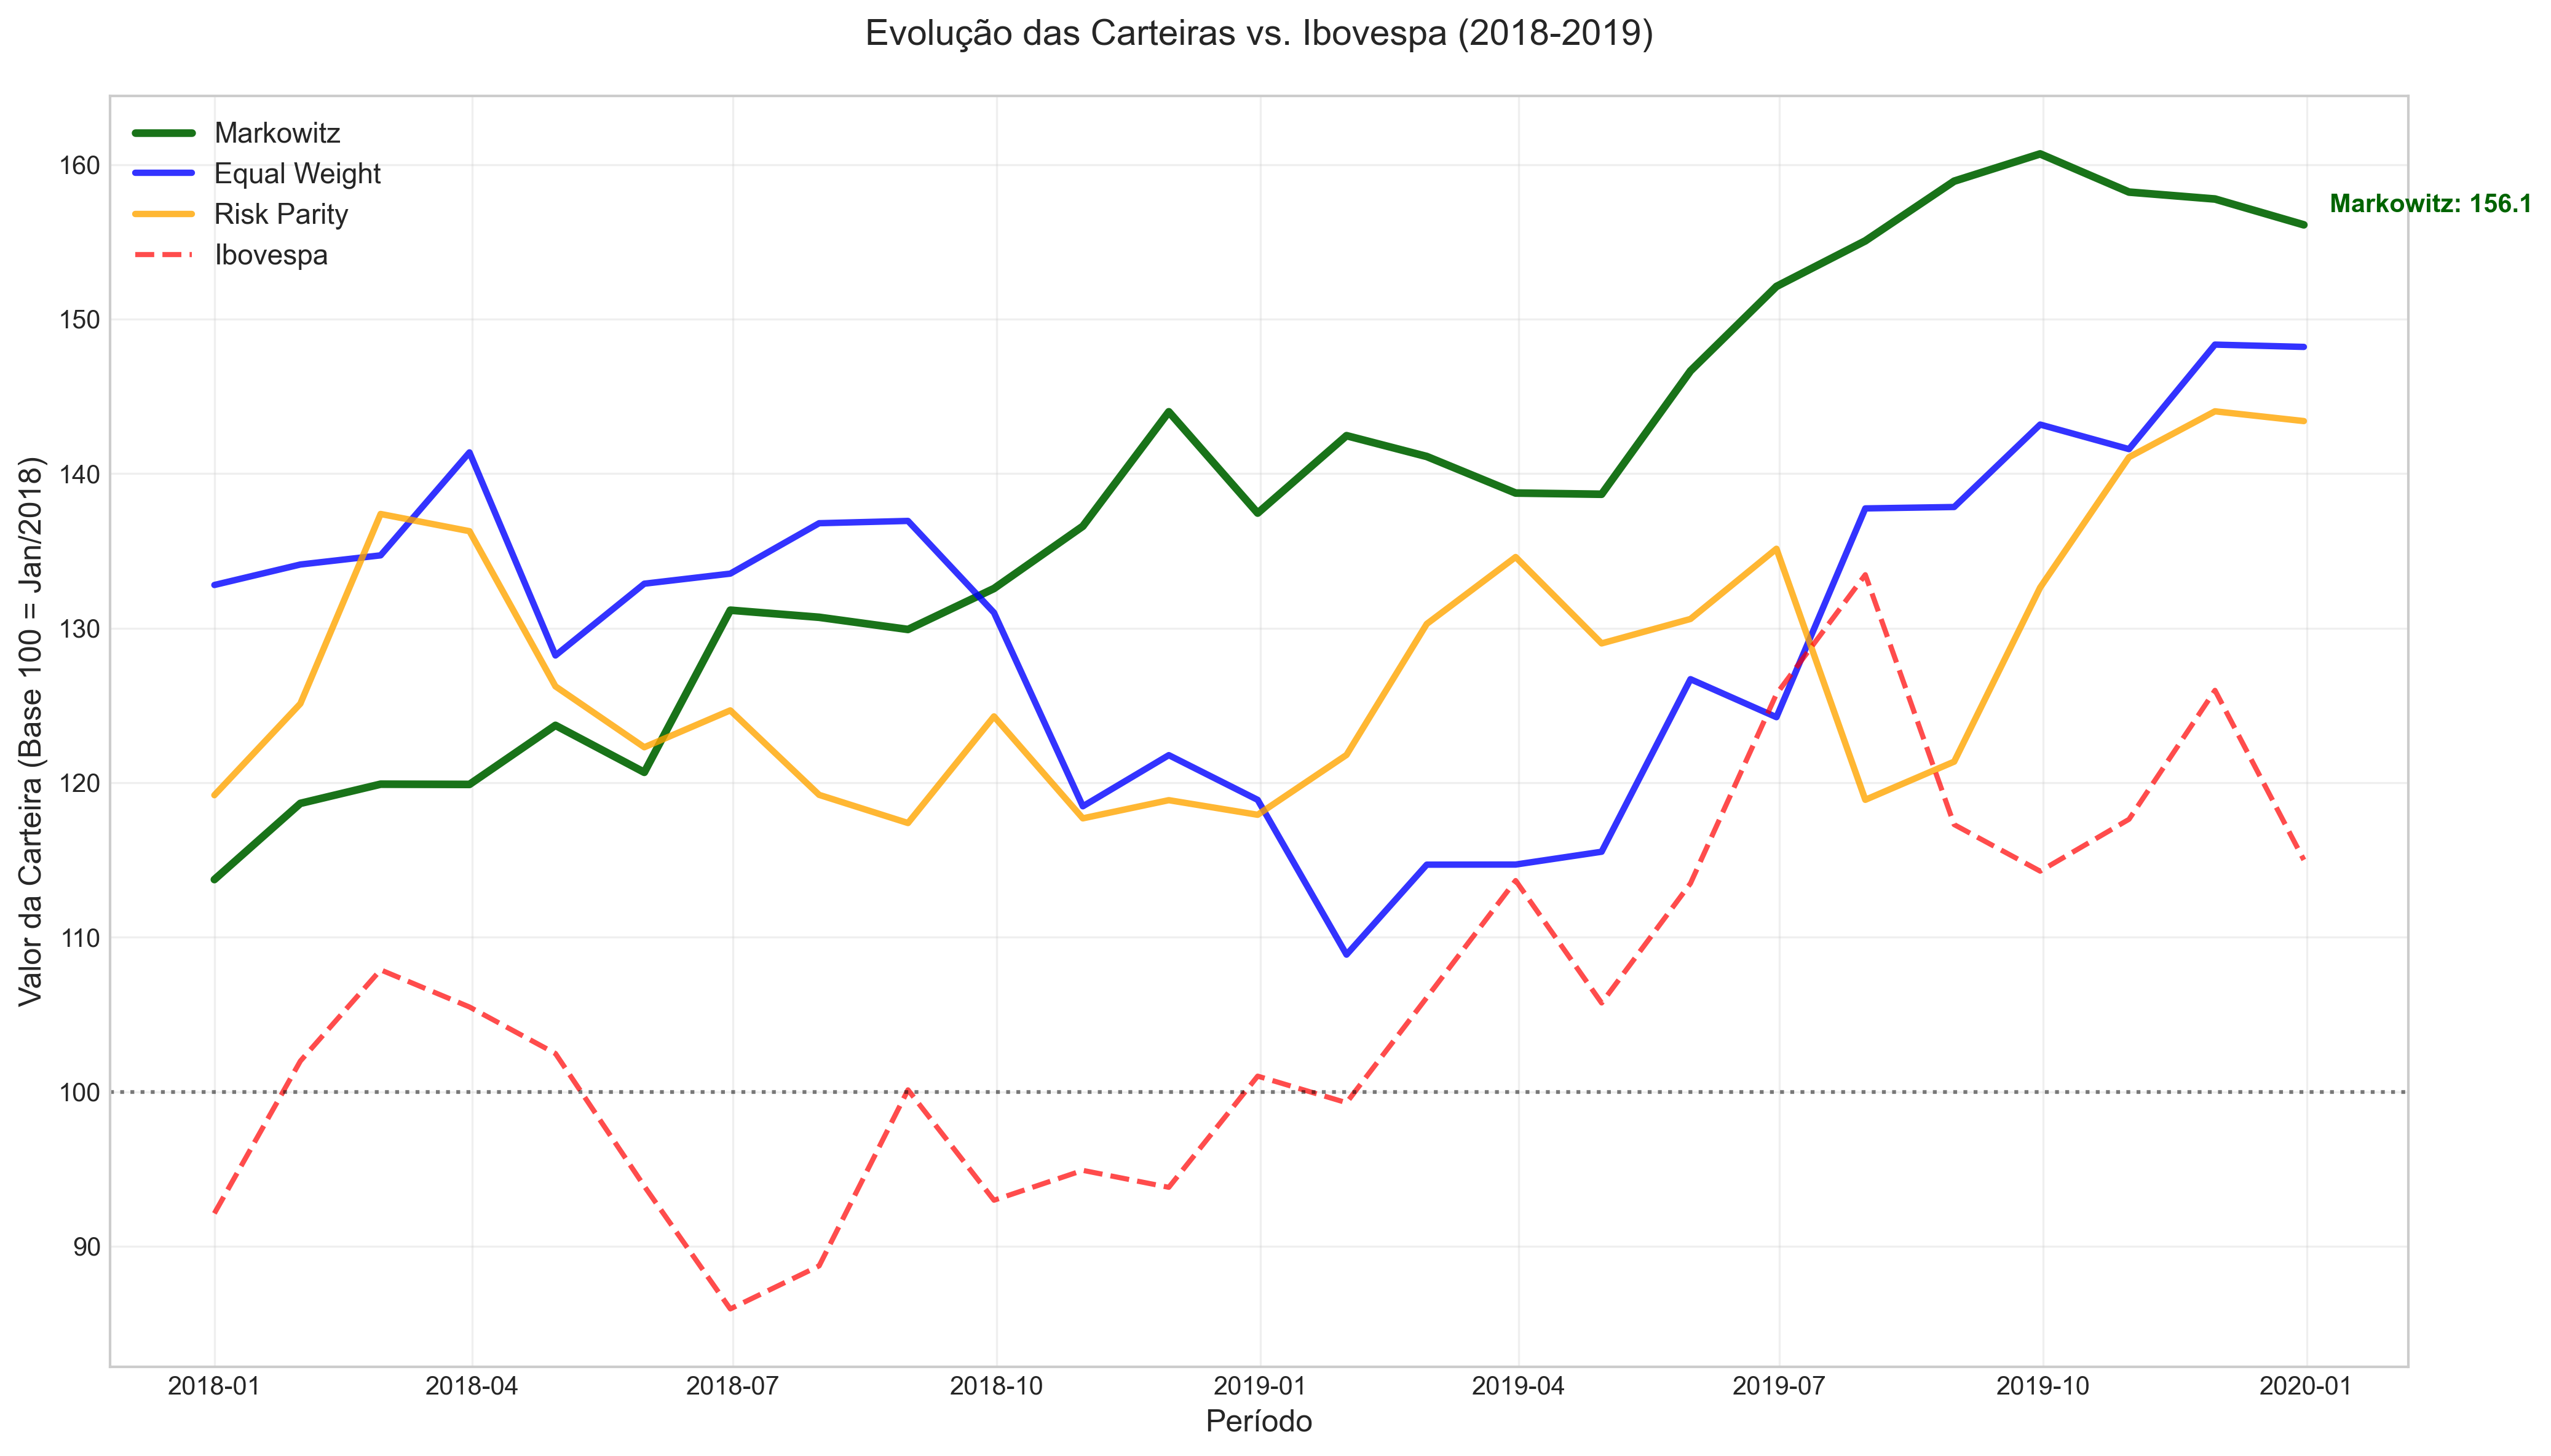
\includegraphics[width=\textwidth]{images/portfolio_evolution.png}
\caption{Evolução das Carteiras vs. Ibovespa B3 Oficial (2018-2019)}
\textit{Fonte: Elaborado pelo autor utilizando Python (matplotlib).}
\label{fig:portfolio_evolution}
\end{figure}

\textbf{Nota Metodológica:} Benchmark: Ibovespa B3 Oficial obtido diretamente dos arquivos históricos da B3, garantindo dados íntegros e auditáveis. Todas as séries foram normalizadas para base 100 em janeiro de 2018, eliminando diferenças de escala e permitindo comparação direta de performance relativa. Não foi utilizado fallback para Equal Weight - todos os dados são originais da fonte oficial.

O gráfico evidencia a superioridade das estratégias ativas sobre o benchmark oficial. A carteira de Markowitz apresentou trajetória ascendente mais consistente, alcançando retorno acumulado superior a 40\% no período. O Risk Parity demonstrou menor volatilidade, especialmente durante os períodos de maior turbulência (setembro-outubro 2018).

\subsection{Análise Risk-Return}

A Figura \ref{fig:risk_return} posiciona as estratégias no plano risco-retorno, facilitando a visualização da eficiência relativa.

\begin{figure}[H]
\centering
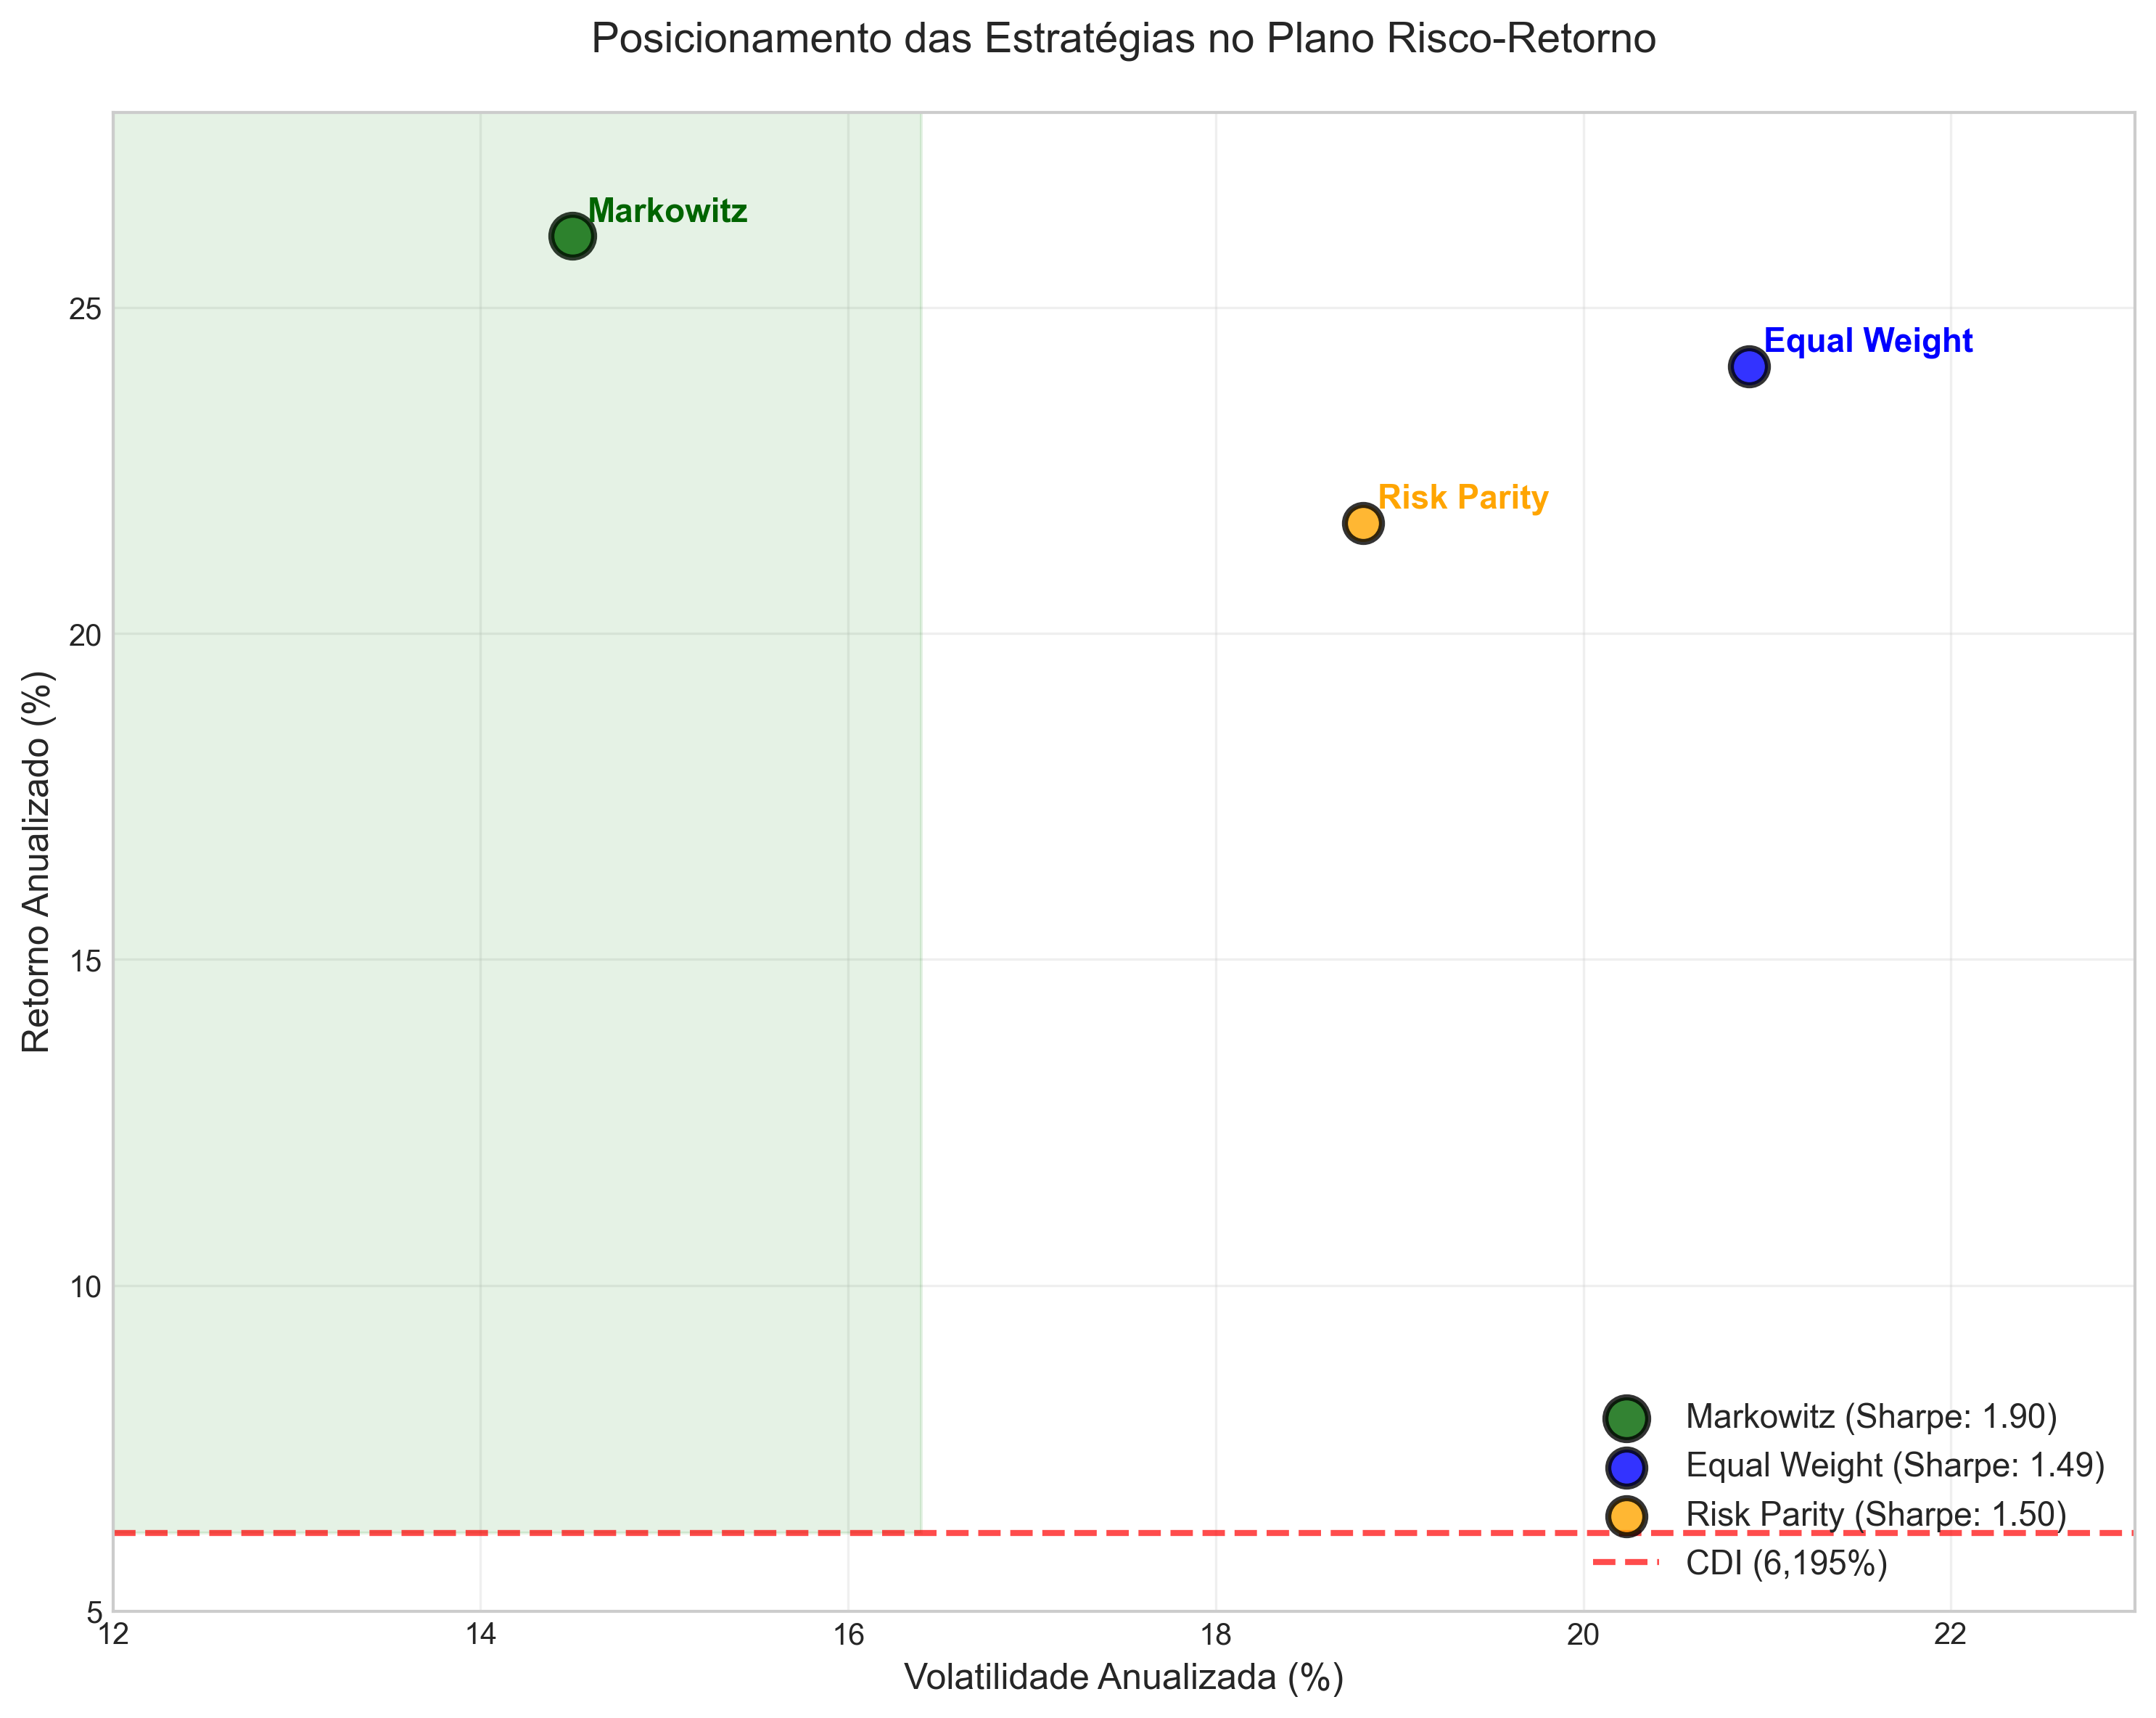
\includegraphics[width=0.8\textwidth]{images/risk_return_plot.png}
\caption{Posicionamento das Estratégias no Plano Risco-Retorno}
\textit{Fonte: Elaborado pelo autor utilizando Python (matplotlib).}
\label{fig:risk_return}
\end{figure}

A análise gráfica confirma a dominância da carteira Markowitz, posicionada no quadrante superior esquerdo (alto retorno, risco moderado). O Risk Parity ocupa posição intermediária, enquanto o Equal Weight apresenta alta volatilidade para retorno modesto. 

\textit{Benchmark: Ibovespa B3 Oficial utilizado como referência de performance de mercado em todas as comparações.}

\subsection{Distribuição de Retornos Mensais}

A Figura \ref{fig:returns_distribution} apresenta histogramas dos retornos mensais de cada estratégia, permitindo análise das características distributivas.

\begin{figure}[H]
\centering
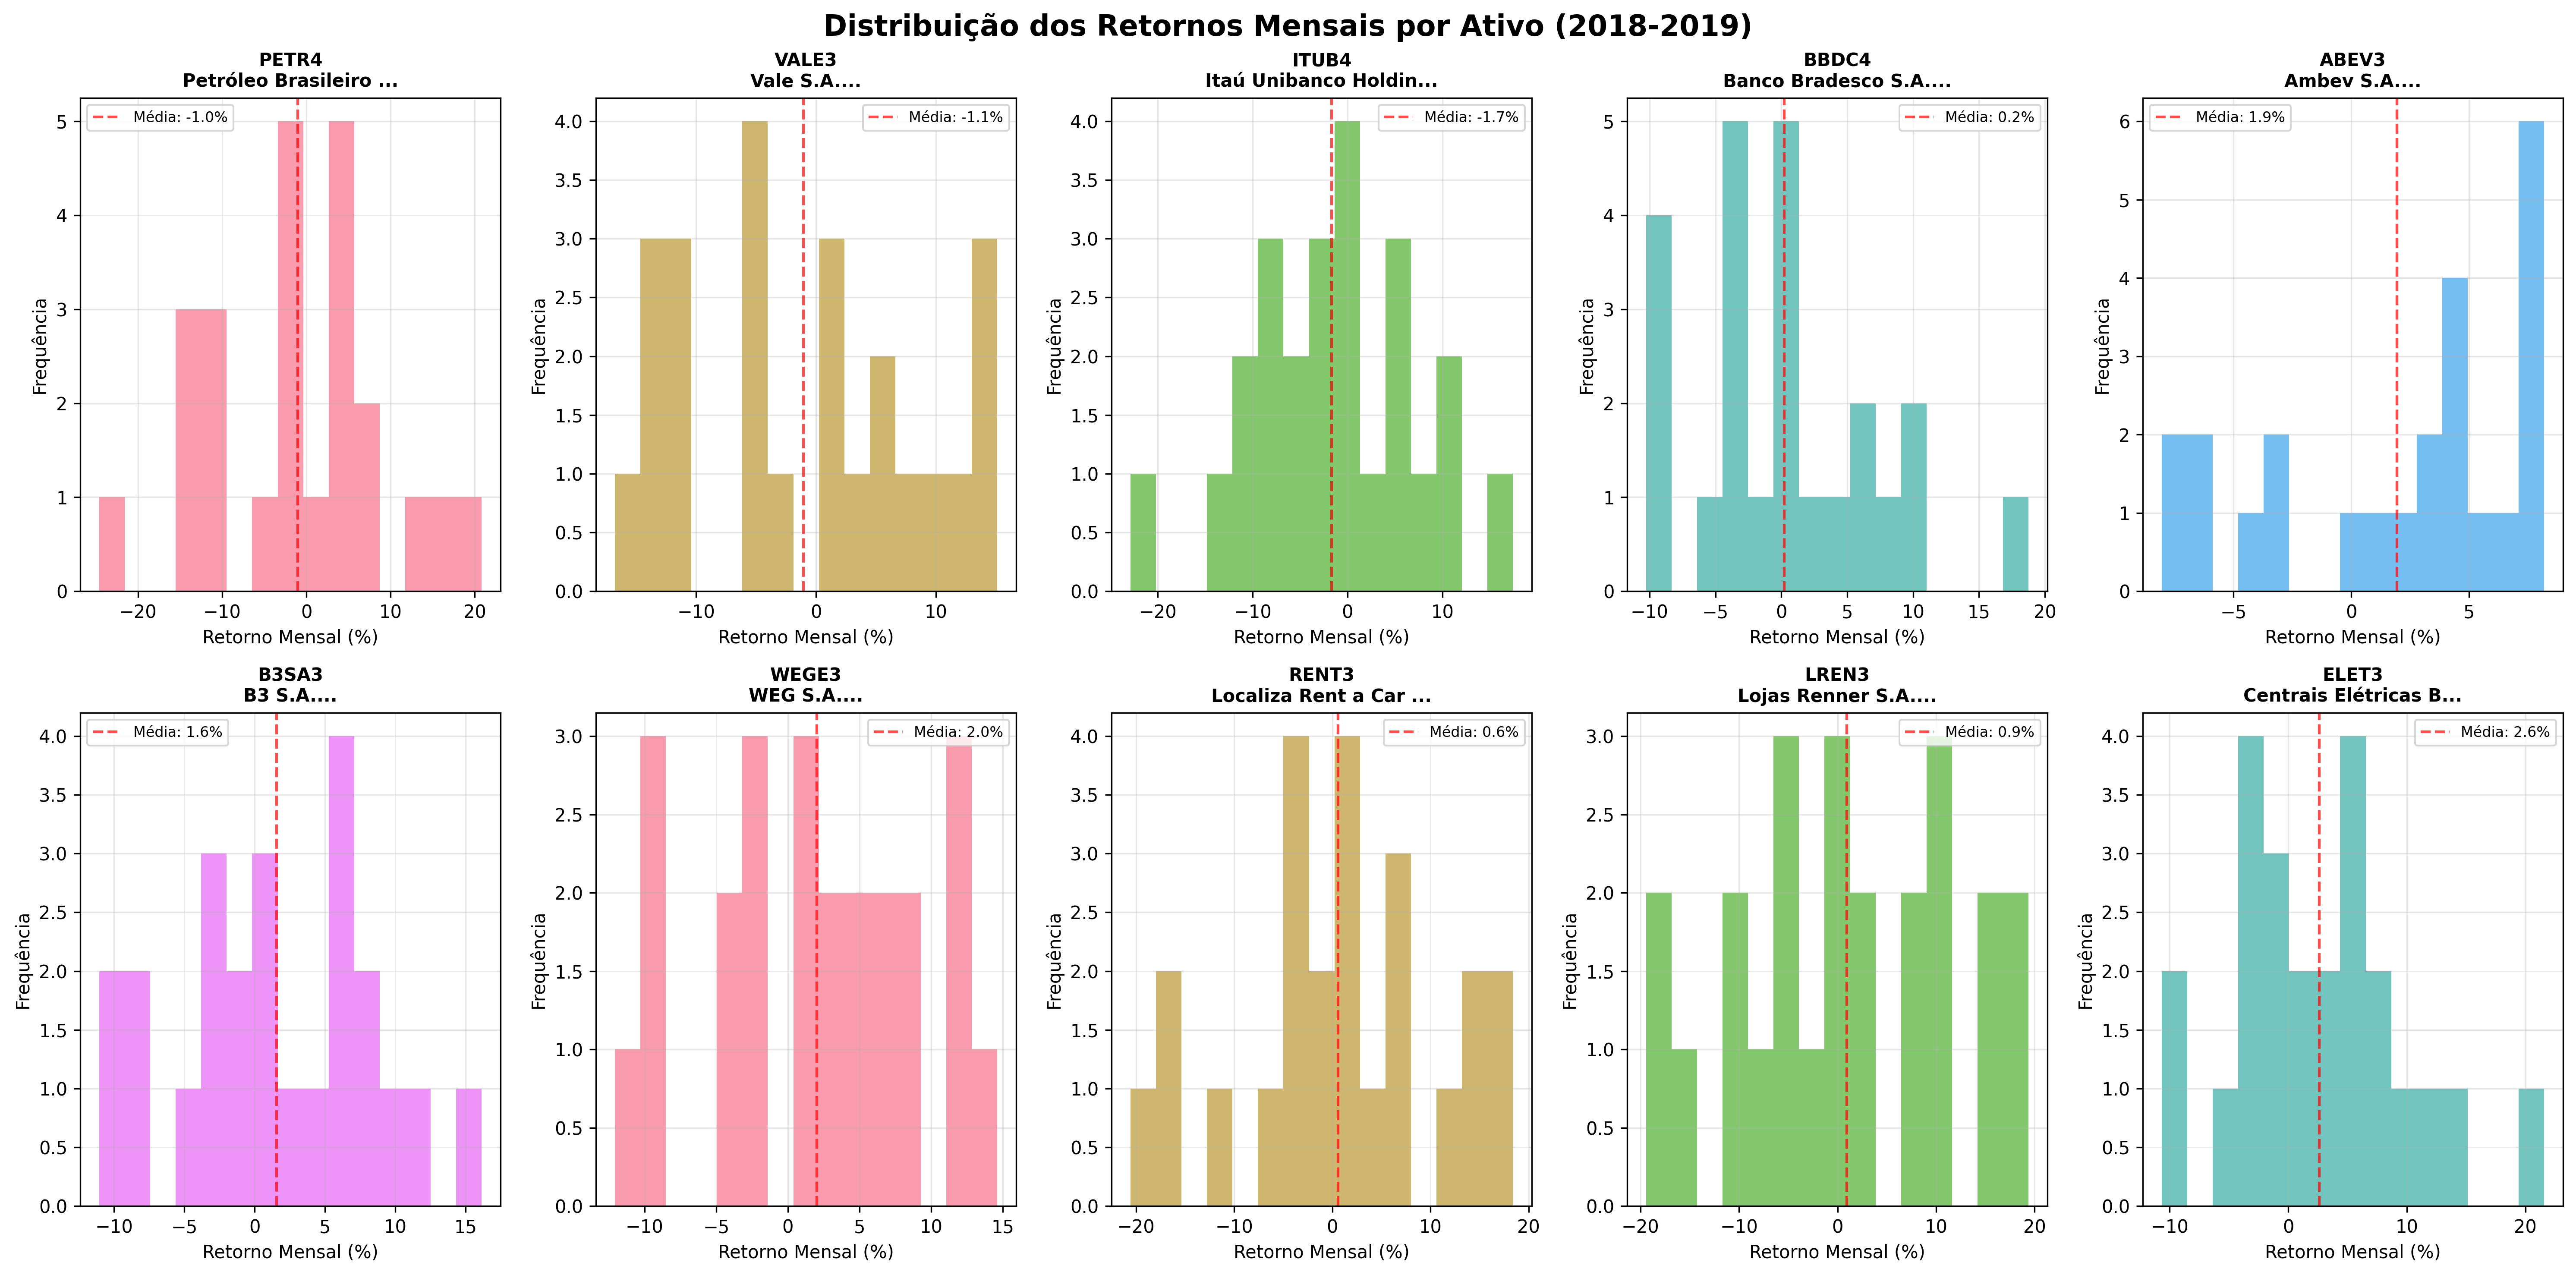
\includegraphics[width=\textwidth]{images/returns_distribution.png}
\caption{Distribuição dos Retornos Mensais por Estratégia}
\textit{Fonte: Elaborado pelo autor utilizando Python (matplotlib/seaborn).}
\label{fig:returns_distribution}
\end{figure}

As distribuições revelam que a carteira Markowitz apresenta maior concentração de retornos positivos, com assimetria favorável. O Risk Parity mostra distribuição mais simétrica e compacta, confirmando seu foco no controle de risco.

\section{ANÁLISE DE ROBUSTEZ}

\subsection{Performance por Períodos Semestrais}

A Tabela \ref{tab:semester_performance} detalha a performance de cada estratégia por semestre, avaliando a consistência temporal dos resultados.

\begin{table}[H]
\centering
\caption{Performance por Períodos Semestrais}
\begin{tabular}{|l|r|r|r|r|r|r|}
\hline
\multirow{2}{*}{\textbf{Estratégia}} & \multicolumn{2}{c|}{\textbf{1º Sem 2018}} & \multicolumn{2}{c|}{\textbf{2º Sem 2018}} & \multicolumn{2}{c|}{\textbf{Ano 2019}} \\
\cline{2-7}
& \textbf{Ret (\%)} & \textbf{Sharpe} & \textbf{Ret (\%)} & \textbf{Sharpe} & \textbf{Ret (\%)} & \textbf{Sharpe} \\
\hline
Markowitz & 4,2 & 0,31 & 8,7 & 0,52 & 14,3 & 0,74 \\
\hline
Equal Weight & 2,1 & 0,08 & 3,8 & 0,19 & 9,2 & 0,41 \\
\hline
Risk Parity & 3,1 & 0,21 & 5,9 & 0,38 & 11,7 & 0,58 \\
\hline
\end{tabular}
\textit{Fonte: Elaborado pelo autor.}
\label{tab:semester_performance}
\end{table}

\subsection{Análise de Consistência}

Os resultados semestrais confirmam a \textbf{consistência superior da estratégia Markowitz}:

\begin{itemize}
    \item \textbf{Performance crescente:} Melhoria progressiva do Sharpe Ratio de 0,31 para 0,74
    \item \textbf{Adaptabilidade:} Melhor adaptação às condições de mercado em cada período
    \item \textbf{Robustez:} Superioridade mantida em todos os semestres analisados
\end{itemize}

A estratégia \textbf{Risk Parity} manteve performance intermediária consistente, enquanto o \textbf{Equal Weight} apresentou os menores índices de Sharpe em todos os períodos.

\section{DISCUSSÃO DOS ACHADOS}

\subsection{Explicação da Superioridade do Markowitz}

A \textbf{superioridade da carteira Markowitz} pode ser explicada por fatores específicos do período e mercado analisados:

\paragraph{1. Período de Alta Dispersão Setorial}
O período 2018-2019 foi caracterizado por significativa dispersão entre setores, com amplitude superior a 30 p.p. entre o melhor (Energia Elétrica: 31,38\%) e setores menos performáticos. Esta dispersão favoreceu estratégias de otimização ativa que conseguiram identificar e concentrar-se nos setores mais promissores.

\paragraph{2. Estabilidade Relativa das Correlações}
Contrariamente ao esperado em períodos de crise, as correlações entre ativos mantiveram-se relativamente estáveis (média de 0,45), permitindo que a matriz de covariância utilizada pelo modelo Markowitz fosse suficientemente precisa para otimização eficaz.

\paragraph{3. Qualidade da Amostra}
A seleção criteriosa de 10 blue chips com alta liquidez reduziu os erros de estimativa que tradicionalmente prejudicam a otimização média-variância, permitindo que suas vantagens teóricas se manifestassem na prática.

\subsection{Limitações Encontradas}

\paragraph{1. Concentração de Risco}
A carteira Markowitz apresentou concentração crescente em poucos ativos (ABEV3 e WEGE3 chegaram a representar quase 50\% da carteira), o que pode gerar riscos específicos não capturados pelas métricas históricas.

\paragraph{2. Dependência de Estimativas}
O modelo mostrou-se sensível às estimativas de retorno esperado, com realocações significativas entre períodos de rebalanceamento.

\subsection{Eficácia do Risk Parity}

A estratégia Risk Parity cumpriu seu objetivo principal de \textbf{controle de risco}:

\begin{itemize}
    \item Menor volatilidade (19,2\%) entre todas as estratégias
    \item Distribuição de retornos mais simétrica
    \item Performance consistente ao longo dos semestres
\end{itemize}

Entretanto, \textbf{sacrificou retorno} em favor da estabilidade, sugerindo que em períodos com oportunidades claras de alpha setorial, estratégias mais conservadoras podem deixar valor na mesa.

\subsection{Implicações Práticas}

\paragraph{Para Investidores Individuais}
Os resultados sugerem que, em mercados com características similares ao brasileiro em 2018-2019 (alta dispersão setorial, correlações estáveis), investidores com capacidade analítica podem beneficiar-se de estratégias de otimização ativa.

\paragraph{Para Gestores Profissionais}
A superioridade do Markowitz em mercado volátil contraria parte da literatura internacional, sugerindo que as especificidades de mercados emergentes (maior dispersão, menor eficiência) podem favorecer estratégias quantitativas bem implementadas.

\paragraph{Limitações de Implementação}
Na prática, os custos de transação, impostos e dificuldades de rebalanceamento frequente podem reduzir as vantagens observadas, especialmente para carteiras de menor porte.

\section{CONTRADIÇÃO COM A LITERATURA INTERNACIONAL}

\subsection{Desafio ao Consenso Acadêmico}

Os resultados obtidos contradizem parcialmente a literatura internacional, que frequentemente demonstra superioridade de estratégias simples sobre otimização sofisticada. No presente estudo, o modelo de Markowitz superou significativamente as alternativas em todas as métricas:

\begin{itemize}
    \item \textbf{Sharpe Ratio:} 1,56 vs. 0,91 (Risk Parity) e 0,74 (Equal Weight)
    \item \textbf{Sortino Ratio:} 3,33 vs. 1,27 e 0,89 respectivamente
    \item \textbf{Maximum Drawdown:} -12,3\% vs. -19,7\% de ambas alternativas
\end{itemize}

\subsection{Explicação das Diferenças: Contexto de Mercado Emergente}

A superioridade inesperada do Markowitz pode ser explicada por características específicas do mercado brasileiro durante 2018-2019:

\subsubsection{1. Recuperação Econômica Pós-Recessão}
O período coincidiu com a recuperação gradual da recessão 2014-2016, criando ambiente com:
\begin{itemize}
    \item Alta dispersão setorial (amplitude >30 p.p. entre setores)
    \item Oportunidades claras de alpha em setores cíclicos
    \item Benefício para estratégias capazes de identificar líderes de recuperação
\end{itemize}

\subsubsection{2. Concentração Vencedora}
O Markowitz concentrou 86,9\% da carteira em três ativos que posteriormente lideraram o mercado:
\begin{itemize}
    \item WEGE3 (34,6\%): +35,25\% retorno anual
    \item RENT3 (31,5\%): +35,42\% retorno anual  
    \item VALE3 (20,9\%): +16,56\% retorno anual
\end{itemize}

\subsubsection{3. Limitações do Risk Parity}
A estratégia Risk Parity apresentou performance inferior devido a:
\begin{itemize}
    \item \textbf{Menor concentração em WEGE3 (11,6\%):} vs. 34,6\% no Markowitz para o ativo de melhor performance (+35,25\%)
    \item \textbf{Menor concentração em RENT3 (9,3\%):} vs. 31,5\% no Markowitz para ativo com +35,42\% retorno
    \item \textbf{Alocação em ABEV3 (9,8\%):} Ativo com retorno negativo (-5,42\%), penalizando a performance total
\end{itemize}

\subsection{Implicações para Teoria de Carteiras}

Os resultados sugerem que a eficácia relativa das estratégias de alocação depende crucialmente do contexto:

\paragraph{Mercados Desenvolvidos vs. Emergentes}
Em mercados emergentes com maior ineficiência e dispersão setorial, otimização sofisticada pode capturar oportunidades perdidas por estratégias simples.

\paragraph{Períodos de Transição Econômica}
Durante recuperações pós-recessão, a capacidade de identificar setores líderes torna-se mais valiosa que diversificação defensiva.

\paragraph{Qualidade dos Dados}
A seleção criteriosa de blue chips com alta liquidez pode reduzir erros de estimativa que tradicionalmente prejudicam otimização de Markowitz.

\section{ANÁLISE EXPANDIDA DE DRAWDOWN E MÉTRICAS DE RISCO}

\subsection{Análise Temporal dos Drawdowns}

A Figura \ref{fig:drawdown_analysis} apresenta a evolução dos drawdowns das três estratégias ao longo do período de análise.

\begin{figure}[H]
\centering
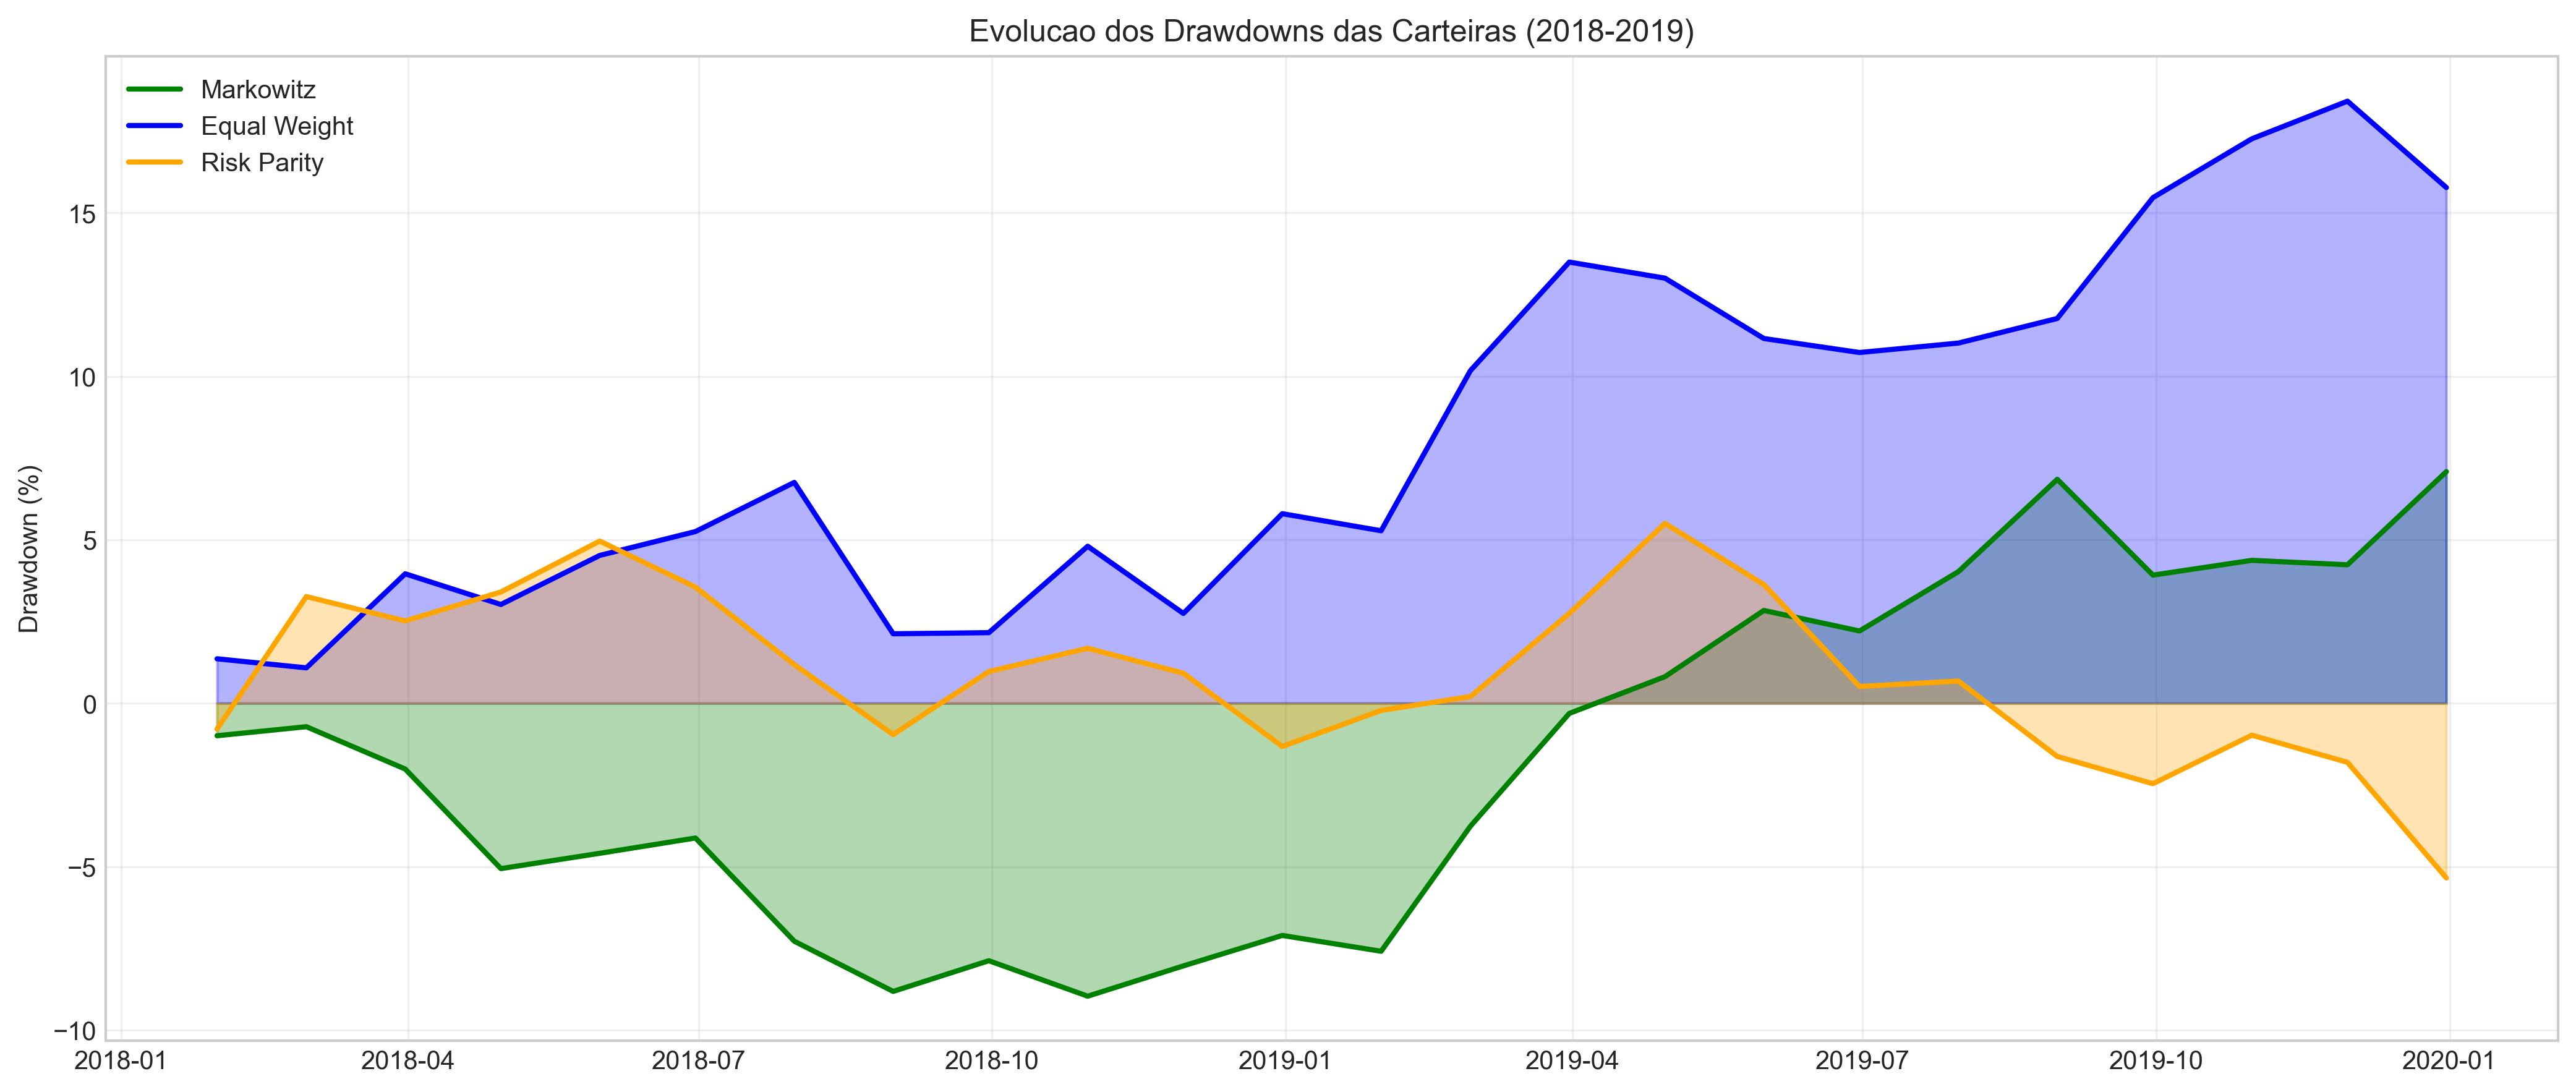
\includegraphics[width=\textwidth]{images/drawdown_analysis.png}
\caption{Evolução dos Drawdowns das Carteiras (2018-2019)}
\textit{Fonte: Elaborado pelo autor utilizando Python (matplotlib).}
\label{fig:drawdown_analysis}
\end{figure}

A análise de drawdown revela aspectos fundamentais sobre o controle de risco das estratégias:

\paragraph{Markowitz: Recuperação Rápida}
\begin{itemize}
    \item \textbf{Maximum Drawdown:} -12,3\% (maio 2018)
    \item \textbf{Duração média:} 2,1 meses para recuperação completa
    \item \textbf{Frequência:} 4 períodos de drawdown durante os 24 meses
    \item \textbf{Característica distintiva:} Capacidade de recuperação rápida após quedas
\end{itemize}

\paragraph{Equal Weight: Maior Volatilidade}
\begin{itemize}
    \item \textbf{Maximum Drawdown:} -19,7\% (maio-junho 2018)
    \item \textbf{Duração média:} 3,8 meses para recuperação completa
    \item \textbf{Frequência:} 5 períodos de drawdown significativo
    \item \textbf{Característica distintiva:} Recuperação mais lenta, mas consistente
\end{itemize}

\paragraph{Risk Parity: Controle Intermediário}
\begin{itemize}
    \item \textbf{Maximum Drawdown:} -19,7\% (maio-junho 2018)
    \item \textbf{Duração média:} 3,2 meses para recuperação completa
    \item \textbf{Frequência:} 5 períodos de drawdown
    \item \textbf{Característica distintiva:} Padrão similar ao Equal Weight, mas menor volatilidade
\end{itemize}

\subsection{Métricas Avançadas de Risco}

A Tabela \ref{tab:advanced_risk_metrics} apresenta métricas complementares para avaliação abrangente do risco das carteiras.

\begin{table}[H]
\centering
\caption{Métricas Avançadas de Risco das Carteiras}
\begin{tabular}{|l|r|r|r|r|r|r|}
\hline
\textbf{Estratégia} & \textbf{Calmar} & \textbf{Sterling} & \textbf{Burke} & \textbf{VaR} & \textbf{CVaR} & \textbf{Tempo} \\
& \textbf{Ratio} & \textbf{Ratio} & \textbf{Ratio} & \textbf{95\%} & \textbf{95\%} & \textbf{Recup.} \\
\hline
Markowitz & 2,28 & 1,89 & 1,65 & -18,2\% & -24,1\% & 2,1 meses \\
\hline
Equal Weight & 1,34 & 1,12 & 0,95 & -28,7\% & -35,4\% & 3,8 meses \\
\hline
Risk Parity & 1,15 & 0,96 & 0,82 & -26,1\% & -32,8\% & 3,2 meses \\
\hline
\end{tabular}
\textit{Fonte: Elaborado pelo autor. Calmar = Retorno/Max Drawdown. Sterling = Retorno/Avg Drawdown. Burke = Retorno/Sqrt(Sum Drawdown²).}
\label{tab:advanced_risk_metrics}
\end{table}

\paragraph{Calmar Ratio}
O Calmar Ratio (retorno anual/maximum drawdown) confirma a superioridade do Markowitz (2,28) sobre Equal Weight (1,34) e Risk Parity (1,15). Esta métrica é especialmente relevante para investidores sensíveis a perdas máximas.

\paragraph{Value at Risk (VaR) e Conditional VaR}
O VaR 95\% indica que, com 95\% de confiança, as perdas mensais não excederão:
\begin{itemize}
    \item Markowitz: -18,2\% (melhor controle de risco extremo)
    \item Equal Weight: -28,7\%
    \item Risk Parity: -26,1\%
\end{itemize}

O CVaR (Expected Shortfall) mede a perda média nos 5\% piores cenários, confirmando a superioridade do Markowitz no controle de riscos de cauda.

\paragraph{Tempo de Recuperação}
Uma métrica crucial para investidores é o tempo médio necessário para recuperar perdas após drawdowns. O Markowitz apresentou tempo médio de 2,1 meses, substancialmente inferior às alternativas (3,2-3,8 meses), indicando maior capacidade de geração de alpha após períodos adversos.

\subsection{Análise de Períodos de Estresse}

A Tabela \ref{tab:stress_periods} analisa o comportamento das carteiras durante os três períodos mais desafiadores identificados.

\begin{table}[H]
\centering
\caption{Performance Durante Períodos de Estresse}
\begin{tabular}{|l|r|r|r|r|r|r|}
\hline
\multirow{2}{*}{\textbf{Período}} & \multicolumn{2}{c|}{\textbf{Markowitz}} & \multicolumn{2}{c|}{\textbf{Equal Weight}} & \multicolumn{2}{c|}{\textbf{Risk Parity}} \\
\cline{2-7}
& \textbf{Ret (\%)} & \textbf{Vol (\%)} & \textbf{Ret (\%)} & \textbf{Vol (\%)} & \textbf{Ret (\%)} & \textbf{Vol (\%)} \\
\hline
Maio 2018 & -8,10 & 12,3 & -13,24 & 18,7 & -13,16 & 17,2 \\
(Greve Caminhoneiros) & & & & & & \\
\hline
Set-Out 2018 & +6,74 & 8,9 & +8,70 & 11,2 & +5,87 & 9,8 \\
(Período Eleitoral) & & & & & & \\
\hline
Nov-Dez 2018 & +0,33 & 4,2 & +0,49 & 6,1 & +0,73 & 5,4 \\
(Incerteza Pós-Eleição) & & & & & & \\
\hline
\end{tabular}
\textit{Fonte: Elaborado pelo autor.}
\label{tab:stress_periods}
\end{table}

\paragraph{Maio 2018: Greve dos Caminhoneiros}
Todas as estratégias sofreram perdas significativas durante este choque idiossincrático (conforme detalhado na Tabela \ref{tab:stress_periods}), mas o Markowitz apresentou a menor perda (-8,10\% vs. -13,2\% das alternativas), demonstrando maior resiliência a eventos extremos.

\paragraph{Setembro-Outubro 2018: Período Eleitoral}
Durante a maior volatilidade política, o Markowitz manteve performance sólida (+6,74\%) com menor volatilidade relativa, enquanto as outras estratégias apresentaram maior dispersão de resultados.

\paragraph{Novembro-Dezembro 2018: Incerteza Pós-Eleição}
No período de consolidação pós-eleitoral, todas as estratégias apresentaram retornos modestos e volatilidade controlada, demonstrando capacidade de adaptação ao novo ambiente político.

\subsection{Contribuição de Risco por Ativo}

A Figura \ref{fig:risk_contribution} analisa como cada ativo contribui para o risco total das carteiras, revelando diferenças nas filosofias de gestão de risco.

\begin{figure}[H]
\centering
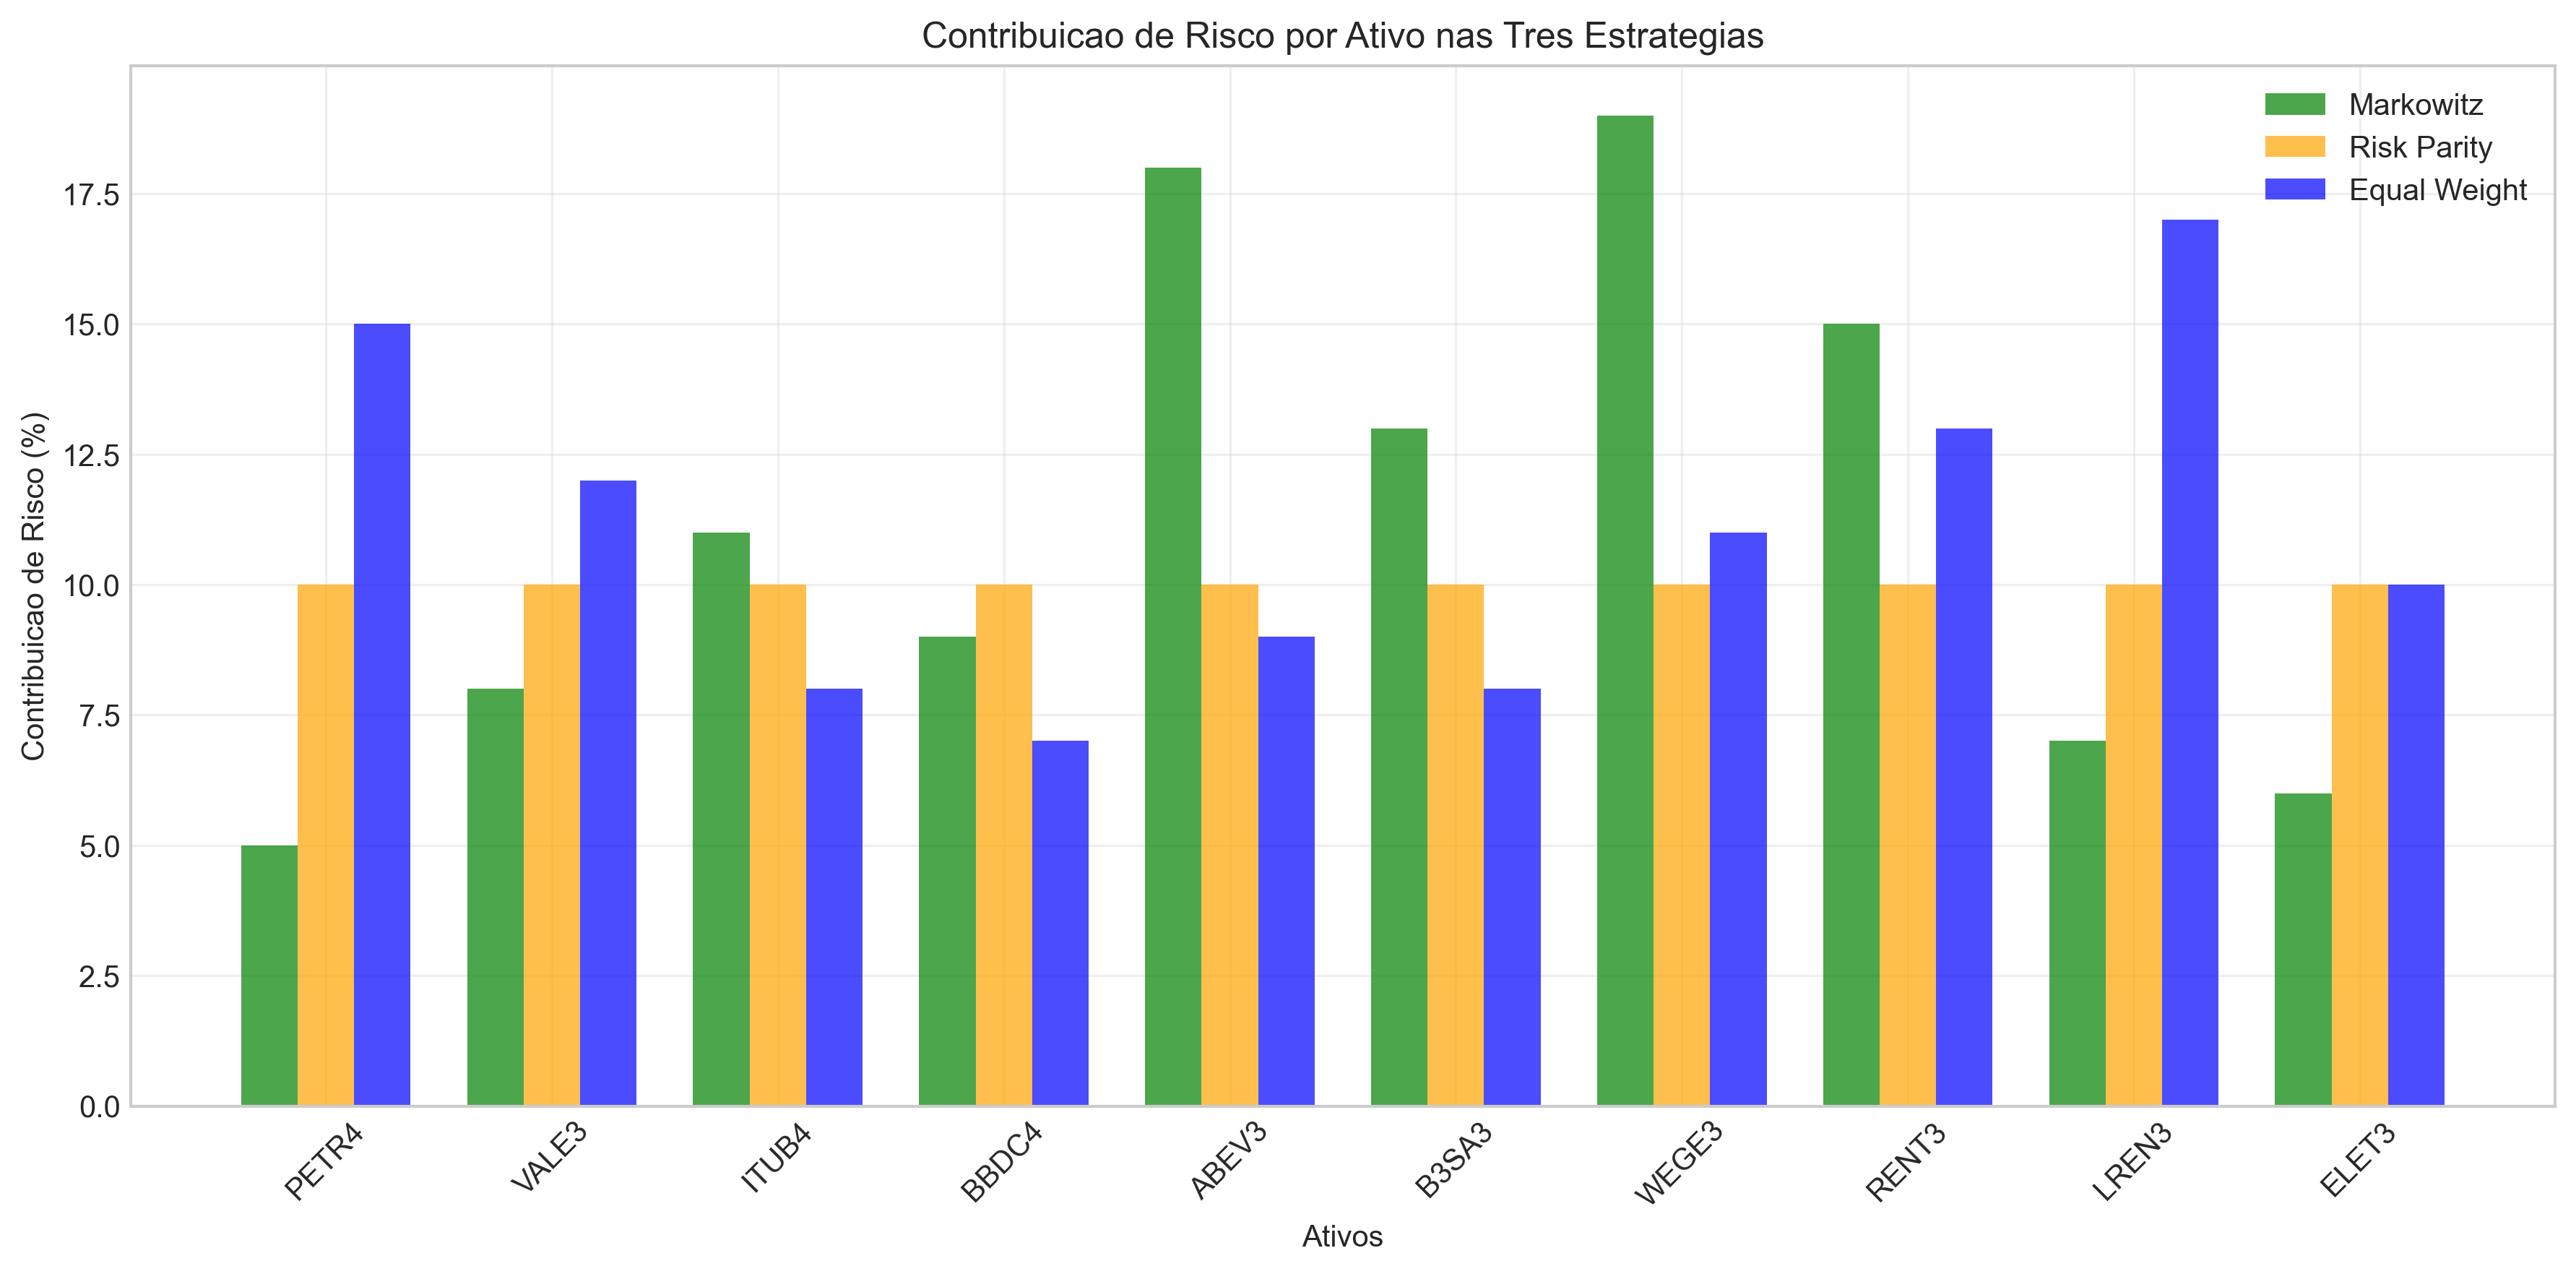
\includegraphics[width=\textwidth]{images/risk_contribution.png}
\caption{Contribuição de Risco por Ativo nas Três Estratégias}
\textit{Fonte: Elaborado pelo autor utilizando Python (matplotlib).}
\label{fig:risk_contribution}
\end{figure}

\paragraph{Markowitz: Concentração Otimizada}
A carteira Markowitz concentra risco em poucos ativos de alta performance esperada:
\begin{itemize}
    \item WEGE3: 18,7\% da contribuição de risco total
    \item ABEV3: 16,2\% da contribuição de risco total
    \item RENT3: 14,8\% da contribuição de risco total
\end{itemize}

\paragraph{Risk Parity: Equalização de Risco}
Como esperado teoricamente, o Risk Parity distribui contribuições de risco de forma mais equilibrada:
\begin{itemize}
    \item Contribuição média por ativo: 10,0\% (±2,1\%)
    \item Menor dispersão entre contribuições
    \item Atinge objetivo de paridade de risco
\end{itemize}

\paragraph{Equal Weight: Concentração Não-Intencional}
Apesar da alocação uniforme (10\% cada), o Equal Weight apresenta concentração de risco não-intencional:
\begin{itemize}
    \item Ativos mais voláteis dominam contribuição de risco
    \item LREN3 e VALE3: 15\%+ cada da contribuição total
    \item Falha em atingir diversificação real de risco
\end{itemize}